\chapter{Evaluation}
\label{chap:evaluation}
in this chapter, we evaluate and compare various different settings

"We found crossover and mutation most influential in GA success."\cite{mills_determining_2015}

"The cross over operator is found to be the most influential parameter in both the case studies, followed by mutation rate, population size for case study-1 and population size and selection process for case study-2. It is evident that the robust GA parameter settings are sensitive"\cite{majumdar_genetic_2015}

\cite{boyabatli_parameter_2004} also suggest a high mutation rate.



It seams like the high variations does not allow for more complex traffic situations, giving a clear priority to pedestrian actions

TODO: chart: emergency break due to pedestrians vs vehicles








\todo{Come up with a better name than "Default" GA}
The three different algorithms that are going to be compared are as follows:
\begin{itemize}
	\item Default Genetic Algorithm - This is using the best settings found in \ref{chap:hyperparameter_tuning:population}, which are:
	\begin{itemize}
		\item Pop: 96, C: 0.8, M: 0.20, TS: 4, Individual Mutation Probability will stay at 0.1. Chromosome Encoding is set to Time and Gene Encoding is set to Integer. No Elite. 
		\item The algorithm will be run 10 times. The Population of 96 needs to be simulated 31 times per run (30 generations + gen 0), which leads to $96 * 31 * 10 = 29,760$ simulations.
	\end{itemize}
	\item Optimized Genetic Algorithm - This is using the recommended settings found in \ref{chap:hyperparameter_tuning:other_parameter}, which are:
	\begin{itemize}
		\item 	which were CrossoverType: Uniform 0.5, CrossoverPropability: 0.9, MutationPropability: 0.3, ChromosomeType: Time+NPC, GeneType: integer encoding, TournamentSize: 4 and IndividualMutationPropability: 0.1 and Elite: 2. 
		\item The algorithm will be run 10 times. The Population of 96 needs to be simulated 31 times per run (30 generations + gen 0), which leads to $96 * 31 * 10 = 29,760$ simulations.
	\end{itemize}
	\item Random Search - Randomly .
	\begin{itemize}
		\item For selecting the actions, the same dict probabilities from ref appendix are used. 
		\item The algorithm will be run $29,760$ tsimes.
	\end{itemize}
\end{itemize}

\section{Start Scenario 1}
First, a comparison of the three algorithms on scenario 1 was made. The results are shown in \ref{figure:sim_1_comparison}.

\begin{figure}[ht] 
	\label{figure:sim_1_comparison}
	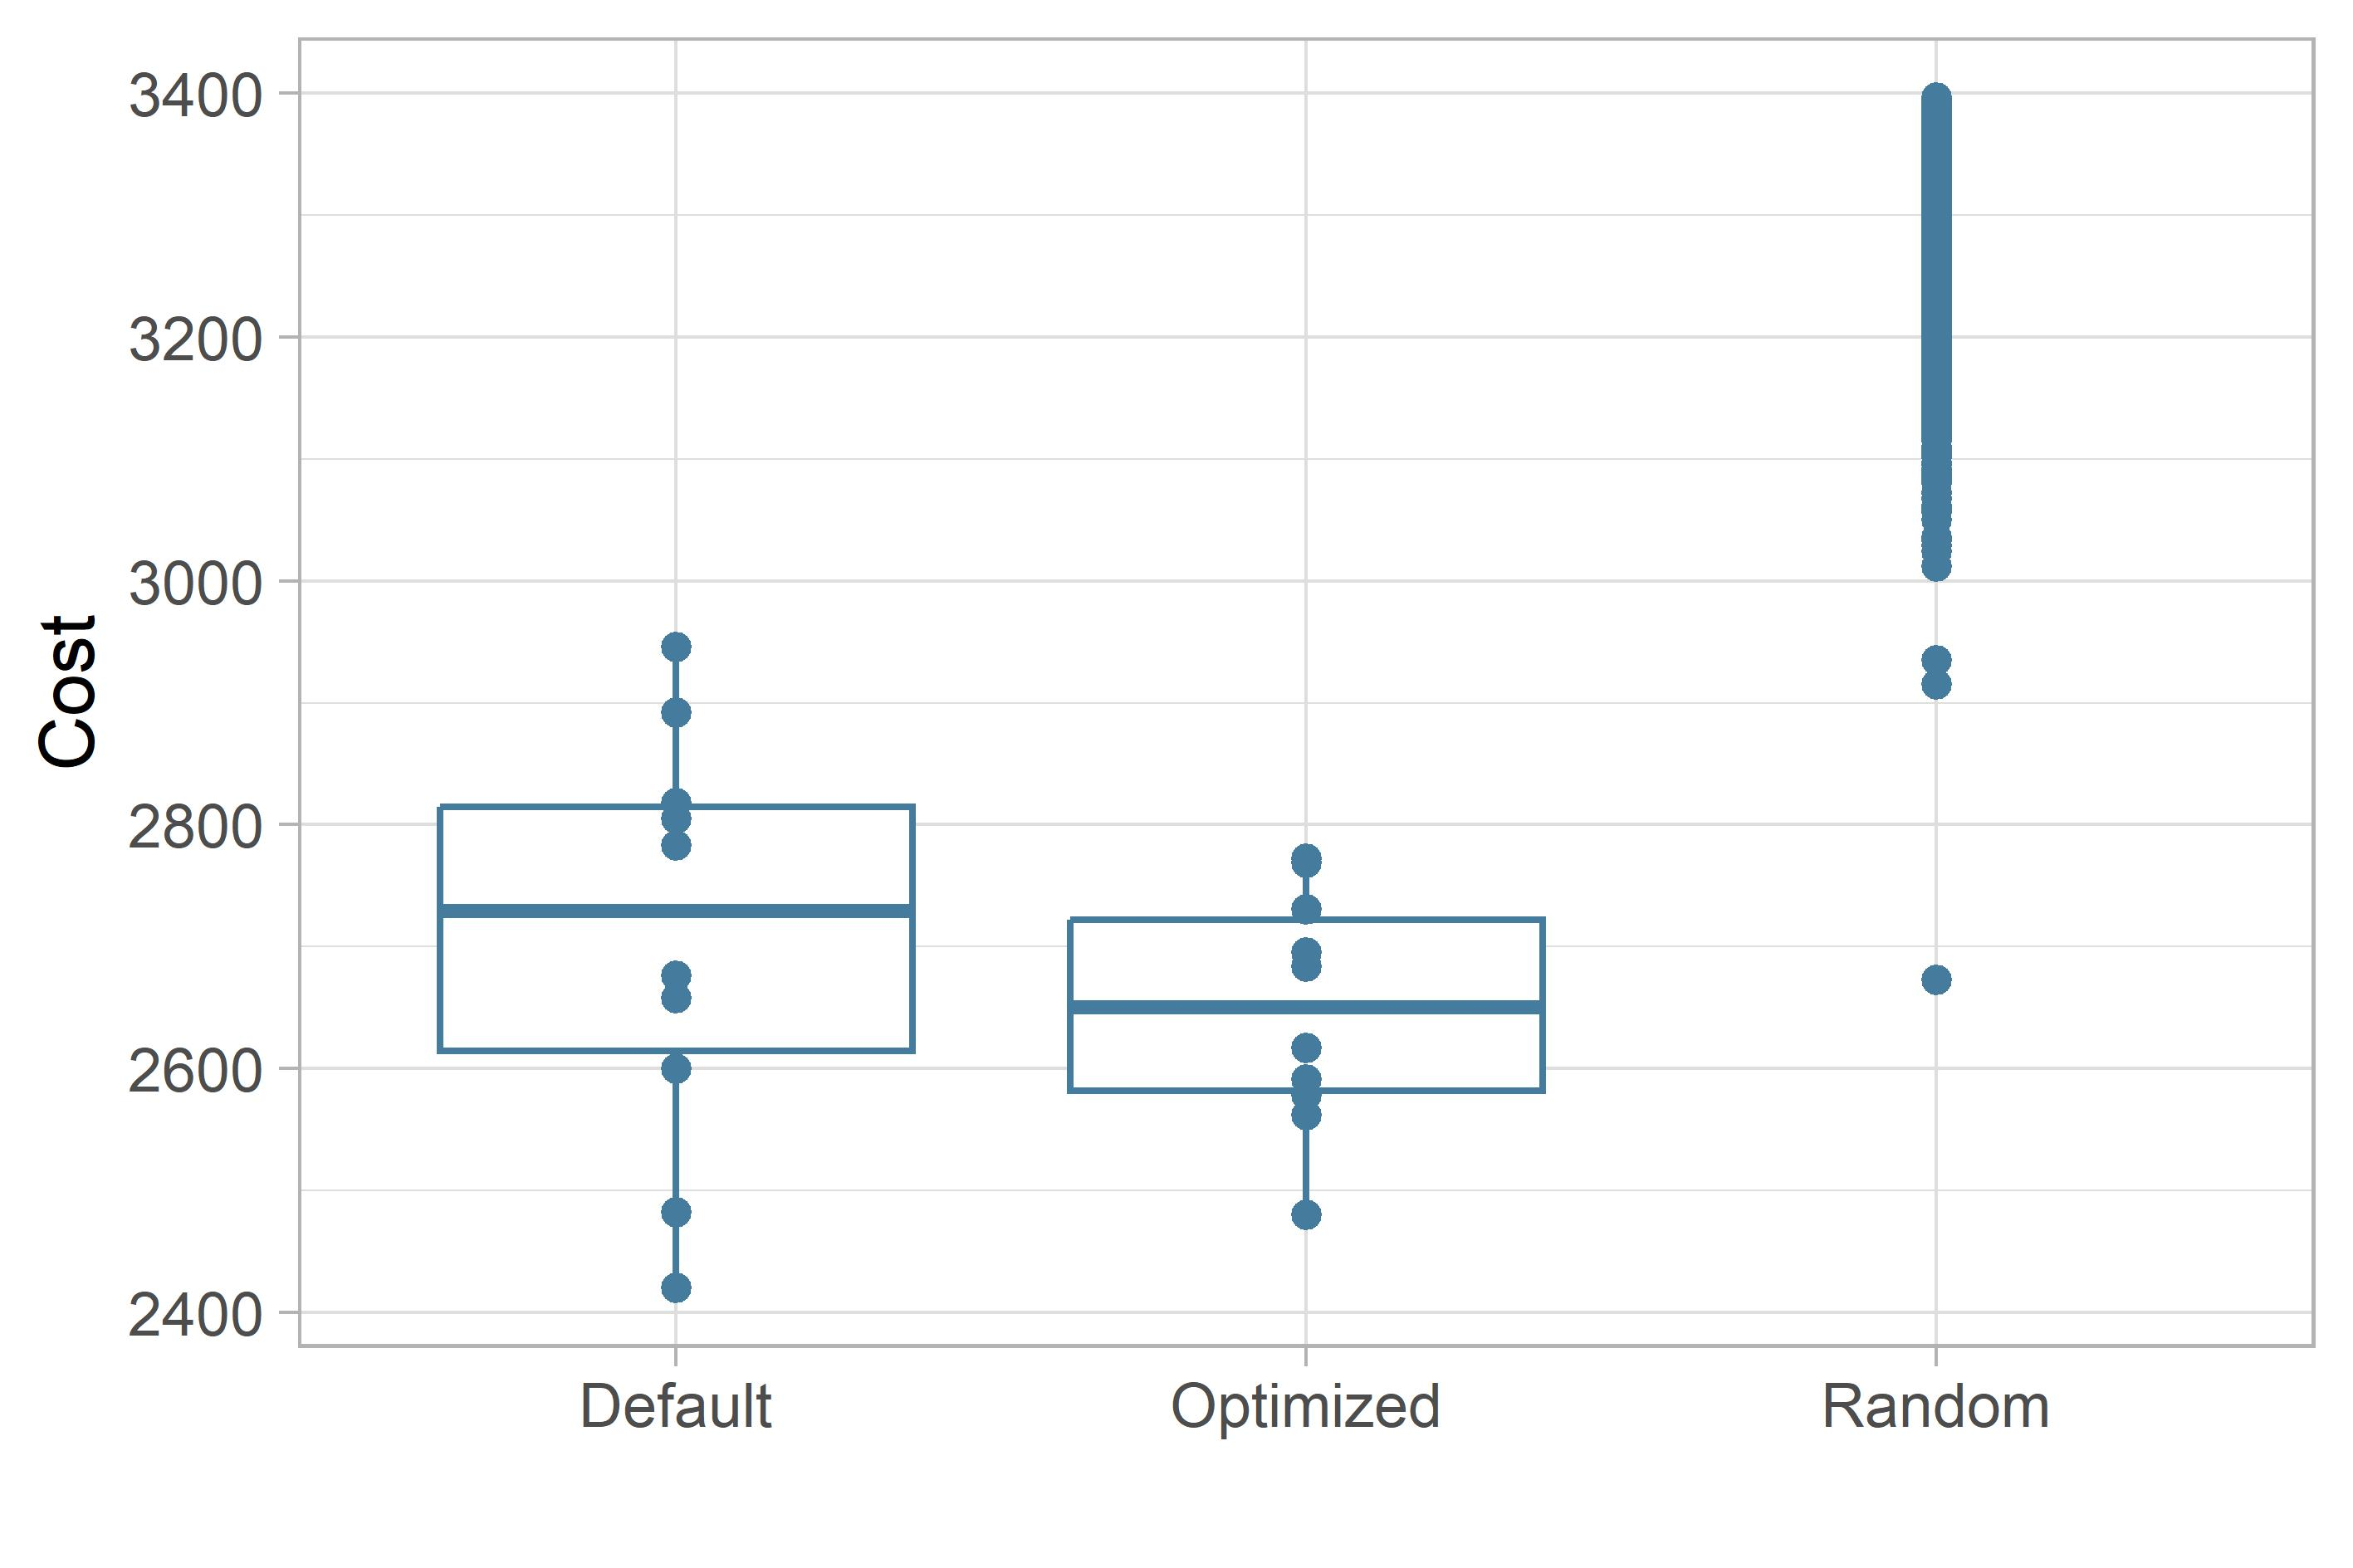
\includegraphics[width=1\linewidth]{simulations/evaluation/plots/sim_1_comparison}
	\caption{Start Scenario 1: Default GA vs Optimized GA vs Random Search}
\end{figure}

Looking at the graph, the Optimized Algorithm clearly outperformed the Default GA as well as Random Search.

Welchs T Test shows a clear result, stating that on average greater fitness is achieved by using Optimized GA (M = 8.52, SE = ?) than from using Default GA (M = 7.09, SE = ?). This difference was significant \textit{t}(17.87) = -3.15, p < .05. It did represent a large effect r = 0.60.
A better performance of the Optimized GA was unsurprising, as it was specifically trained for the used starting scenario.

\todo{Show t test with random}

To further analyse both genetic algorithms, a look at their performance over the generations next to their diversity chart is of interest. Figure \ref{figure:sim_1_ga_comparison} plots the mean over the 10 repetitions, the outline show the min and max values.

\begin{figure}[ht] 
	\label{figure:sim_1_ga_comparison}
	\begin{minipage}[b]{0.5\linewidth}
		\centering
		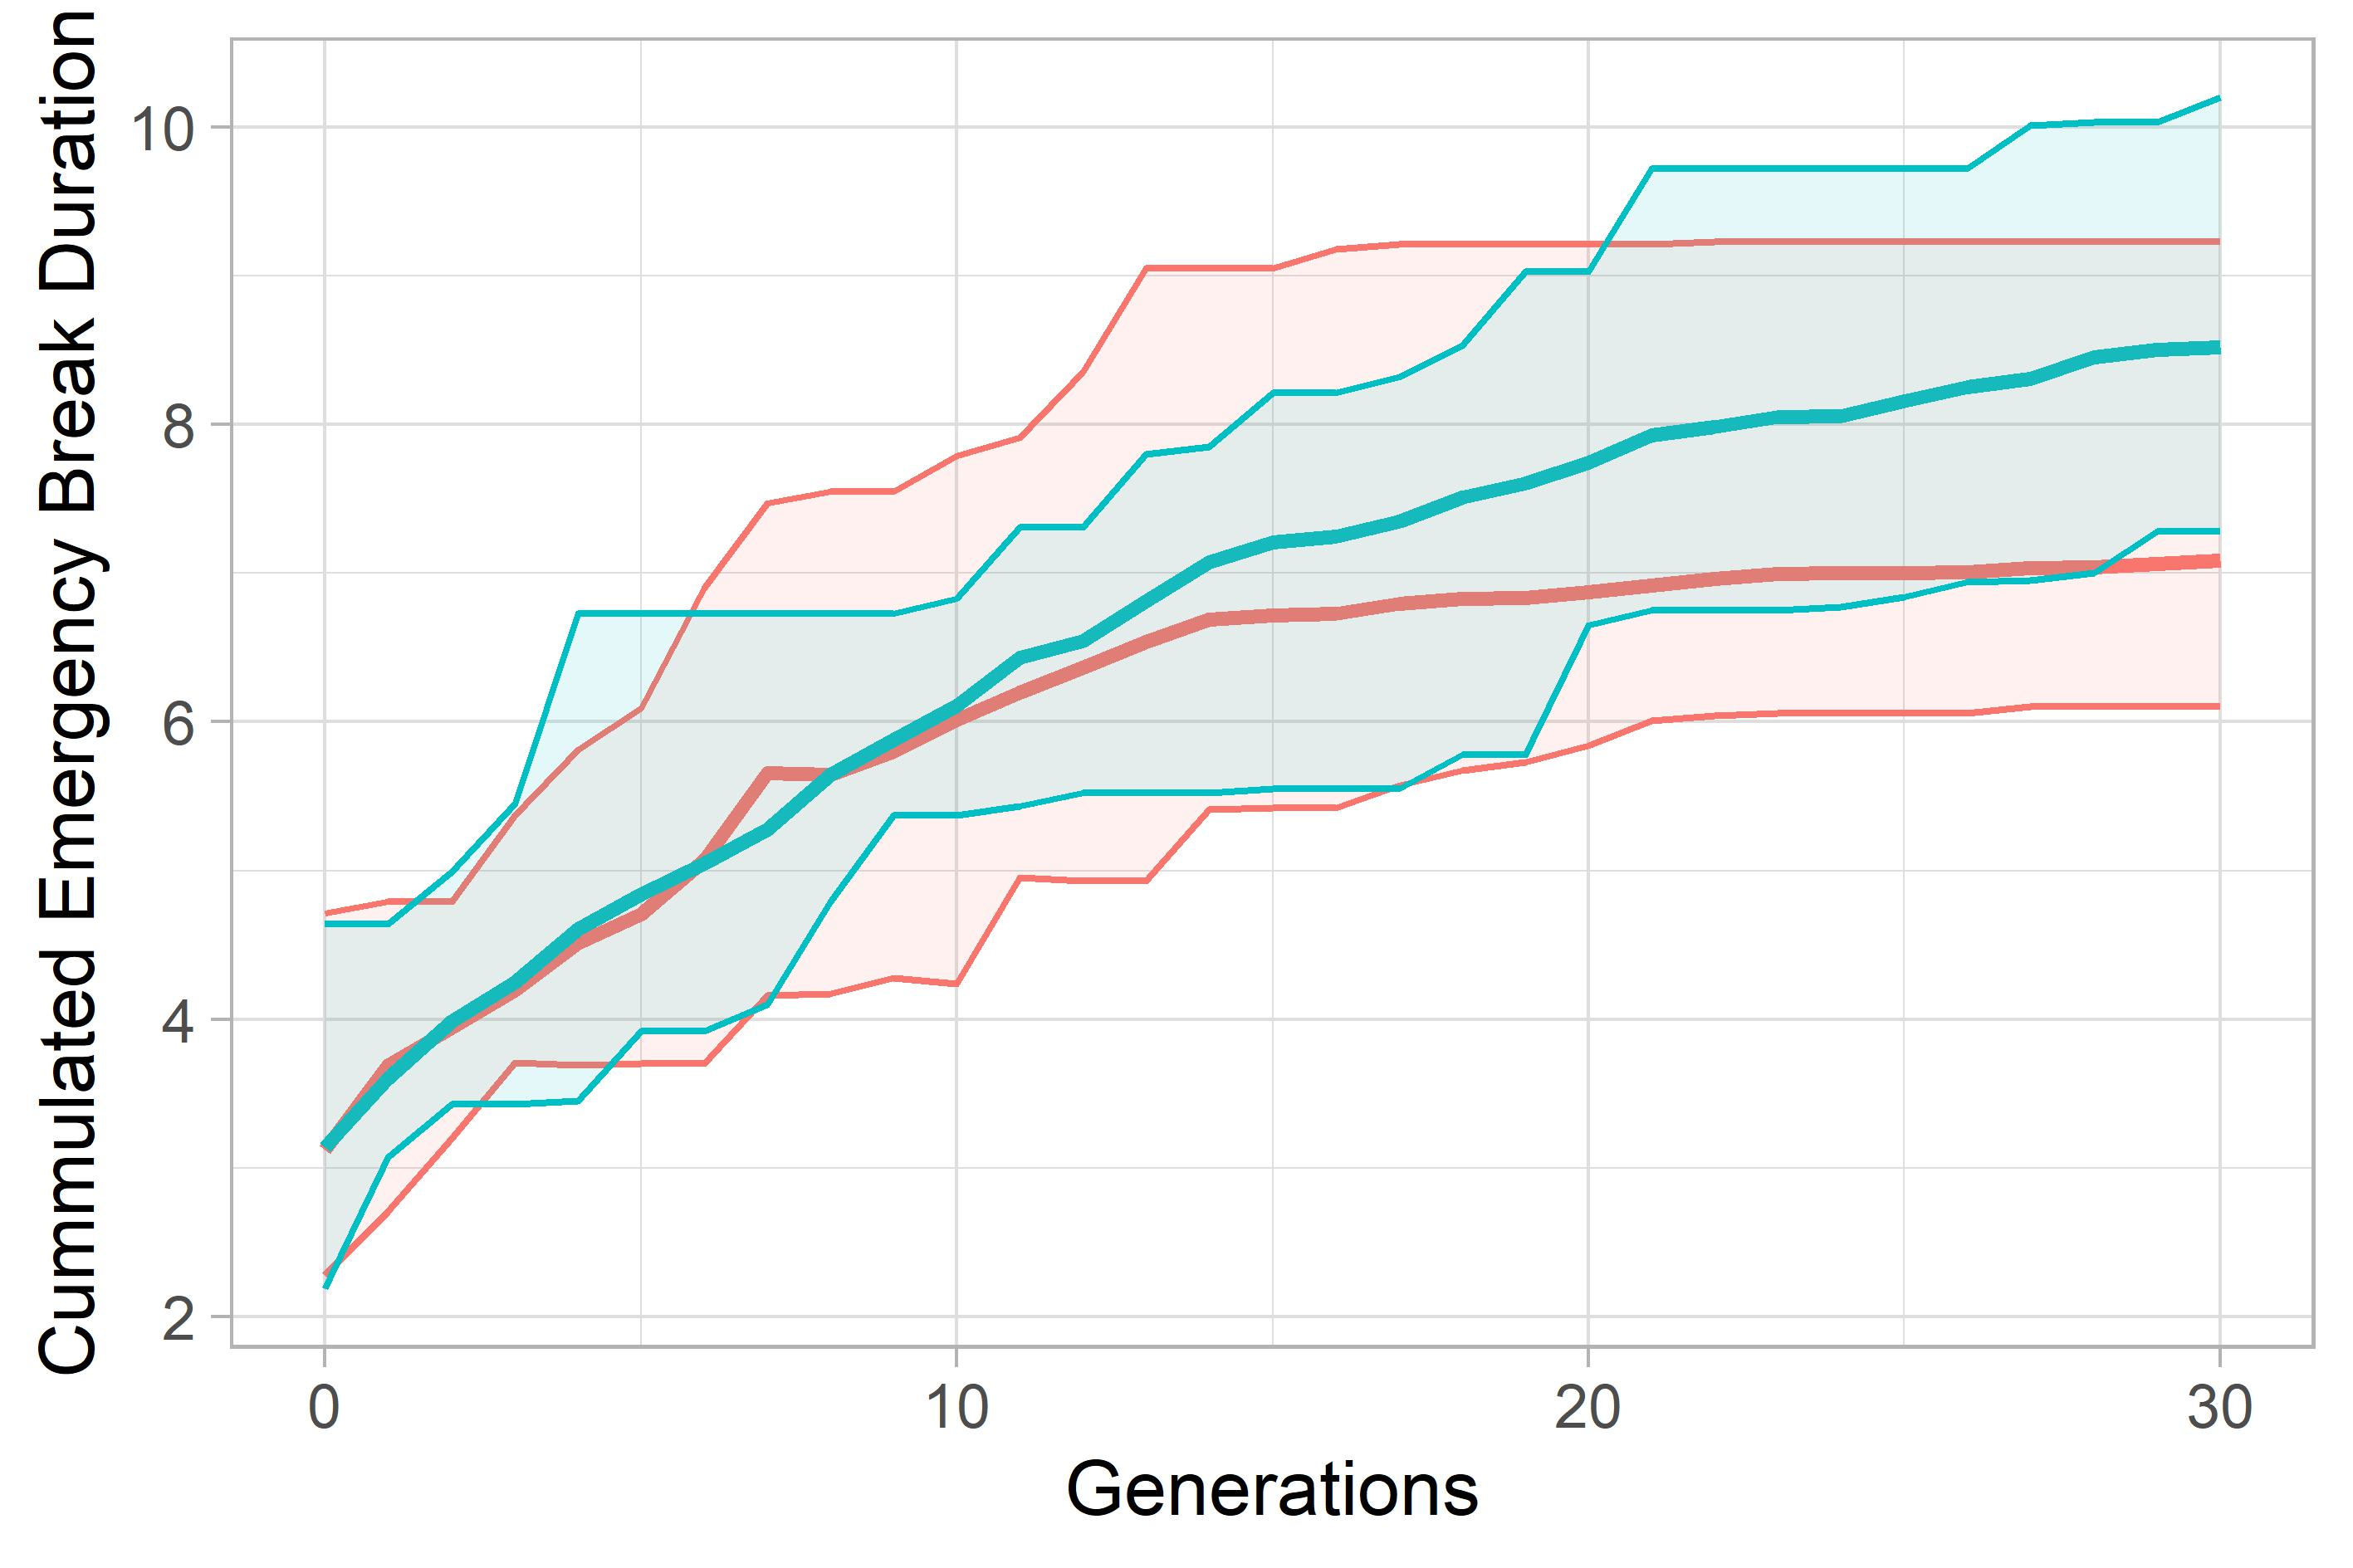
\includegraphics[width=1\linewidth]{simulations/evaluation/plots/sim_1_ga_generations} 
	\end{minipage}%%
	\begin{minipage}[b]{0.5\linewidth}
		\centering
		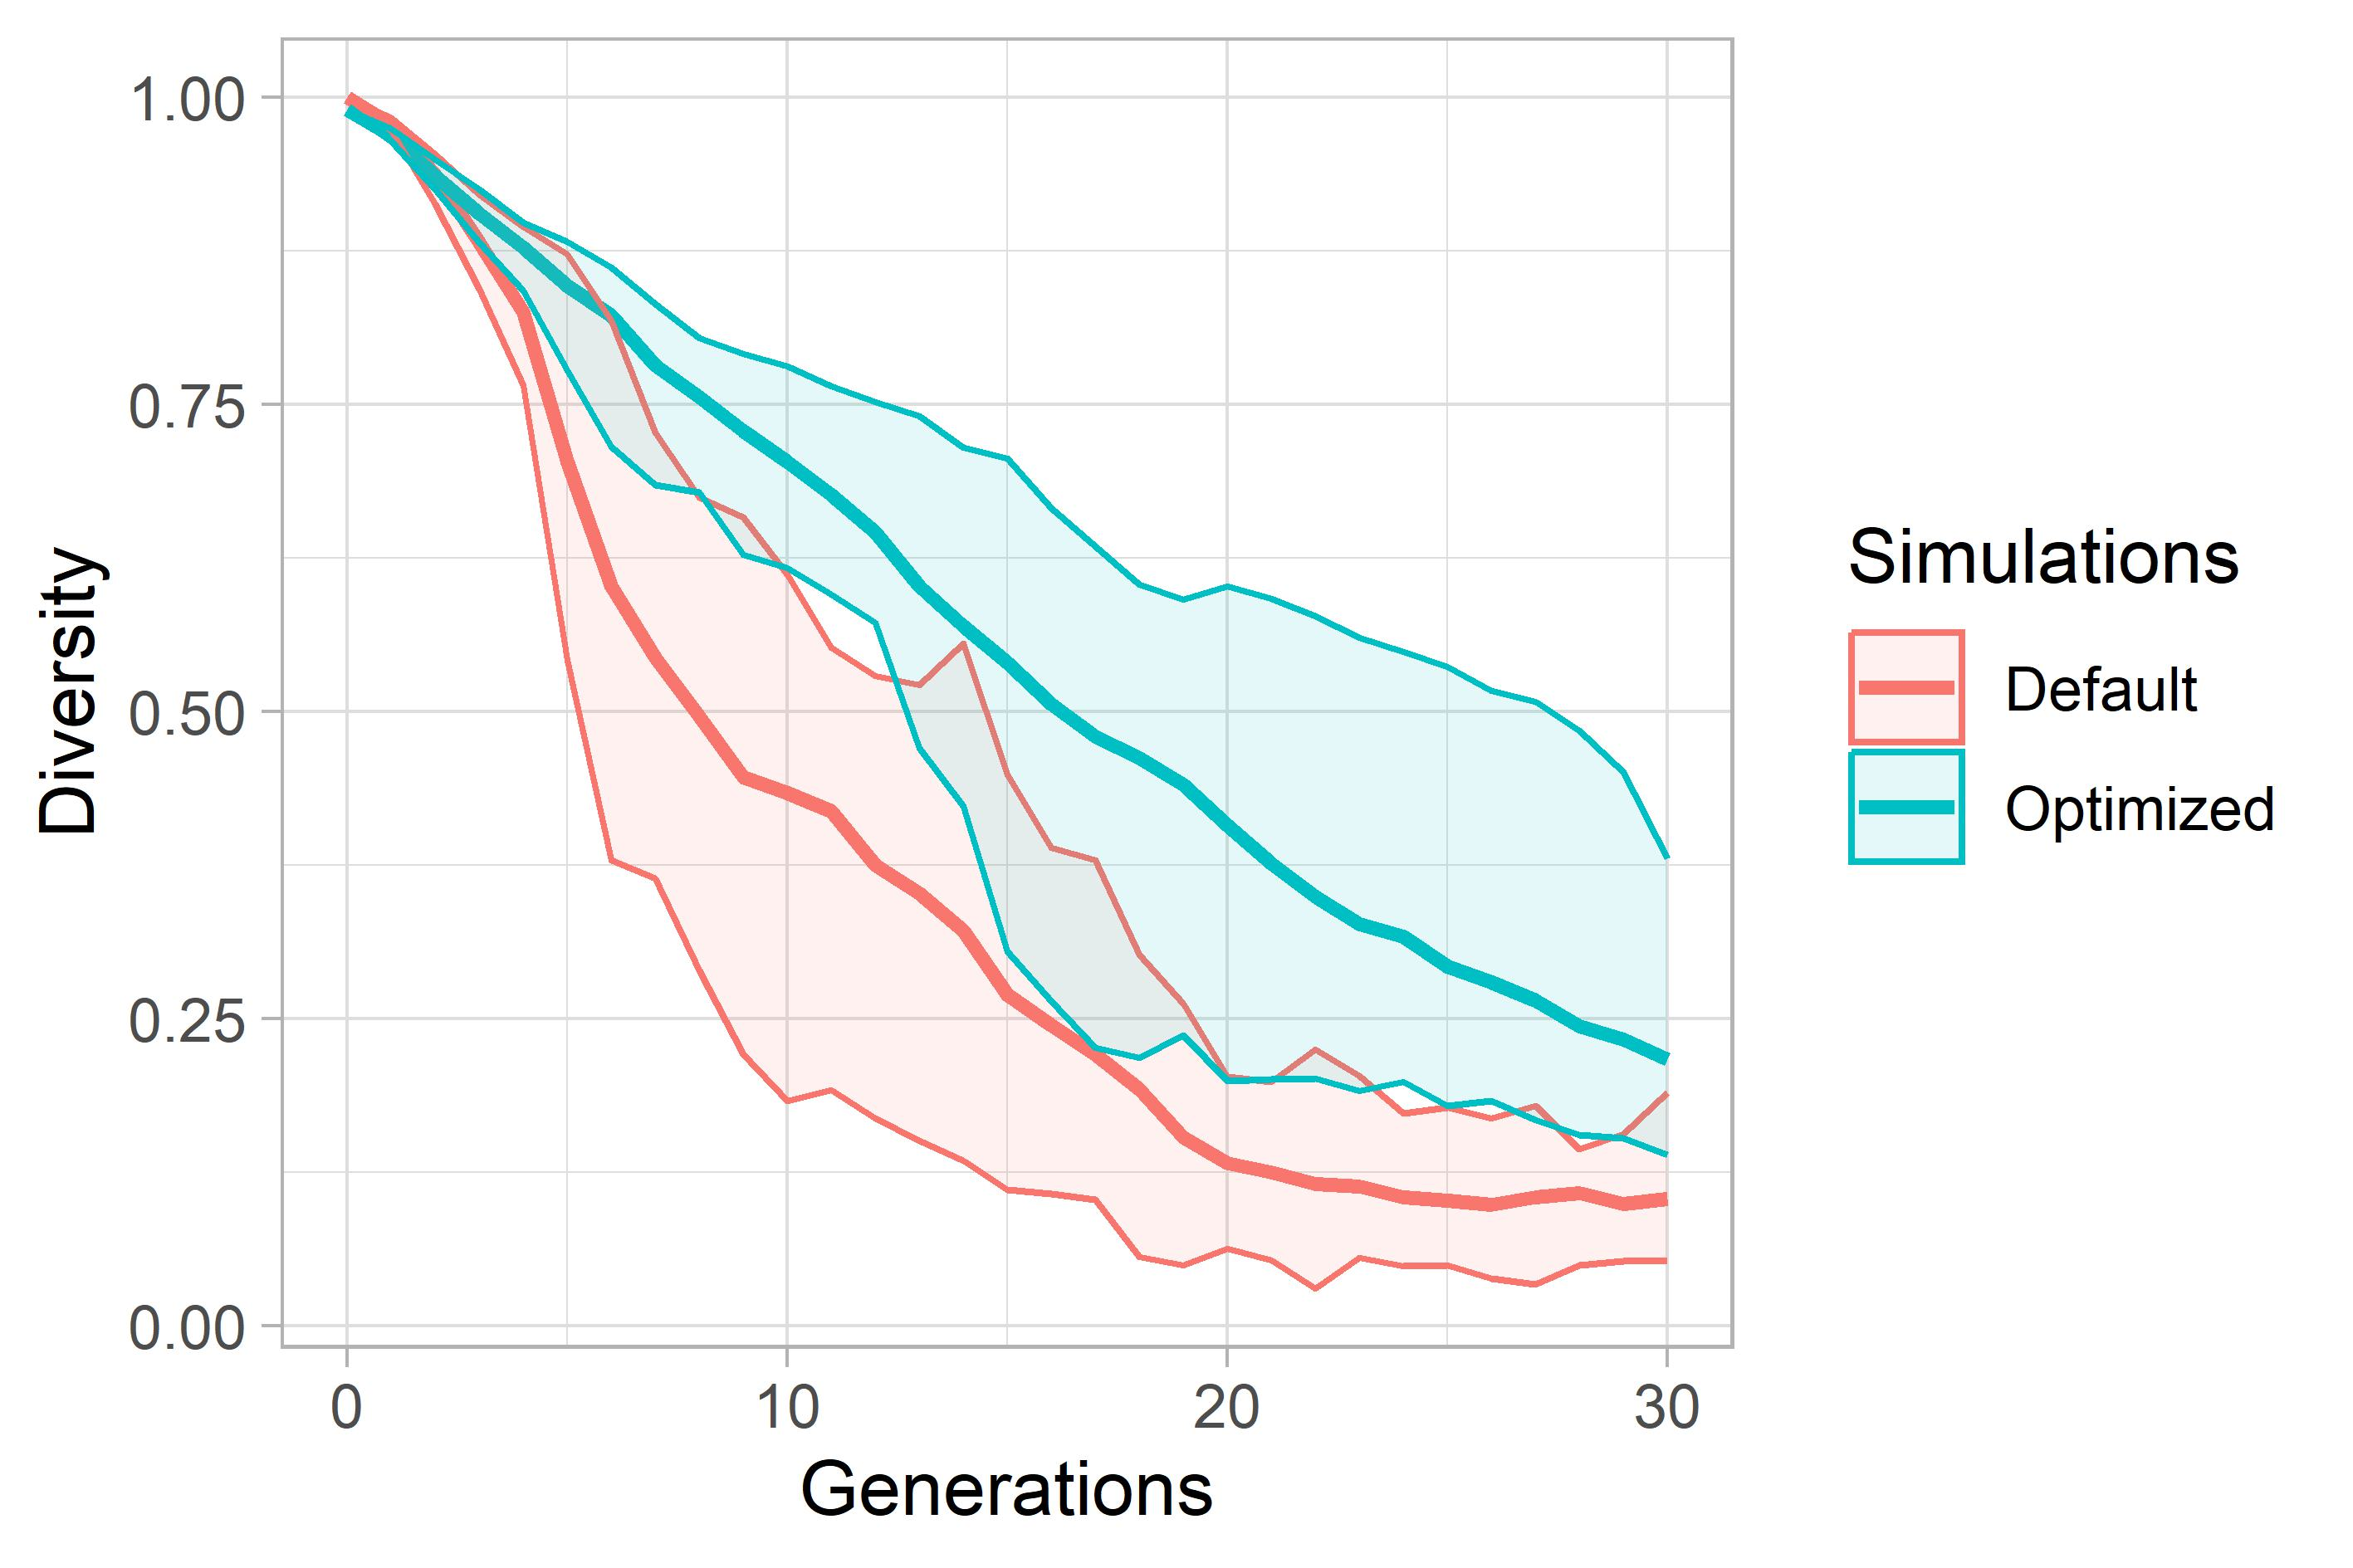
\includegraphics[width=1\linewidth]{simulations/evaluation/plots/sim_1_ga_diversity} 
	\end{minipage} 
	\caption{Start Scenario 1: Comparison of GAs}
\end{figure}

After Generation 10, the rate of improved fitness of the Default GA drops compared to the Optimized one. A combined with an early sharp decline in the diversity, suggests a connection. The optimized GA shows to hold the diversity in the population longer, its rate of convergence is linear.



\section{Start Scenario 2}
scenario 2: 9v 5p
\begin{figure}[ht] 
	\label{figure:sim_2_comparison}
	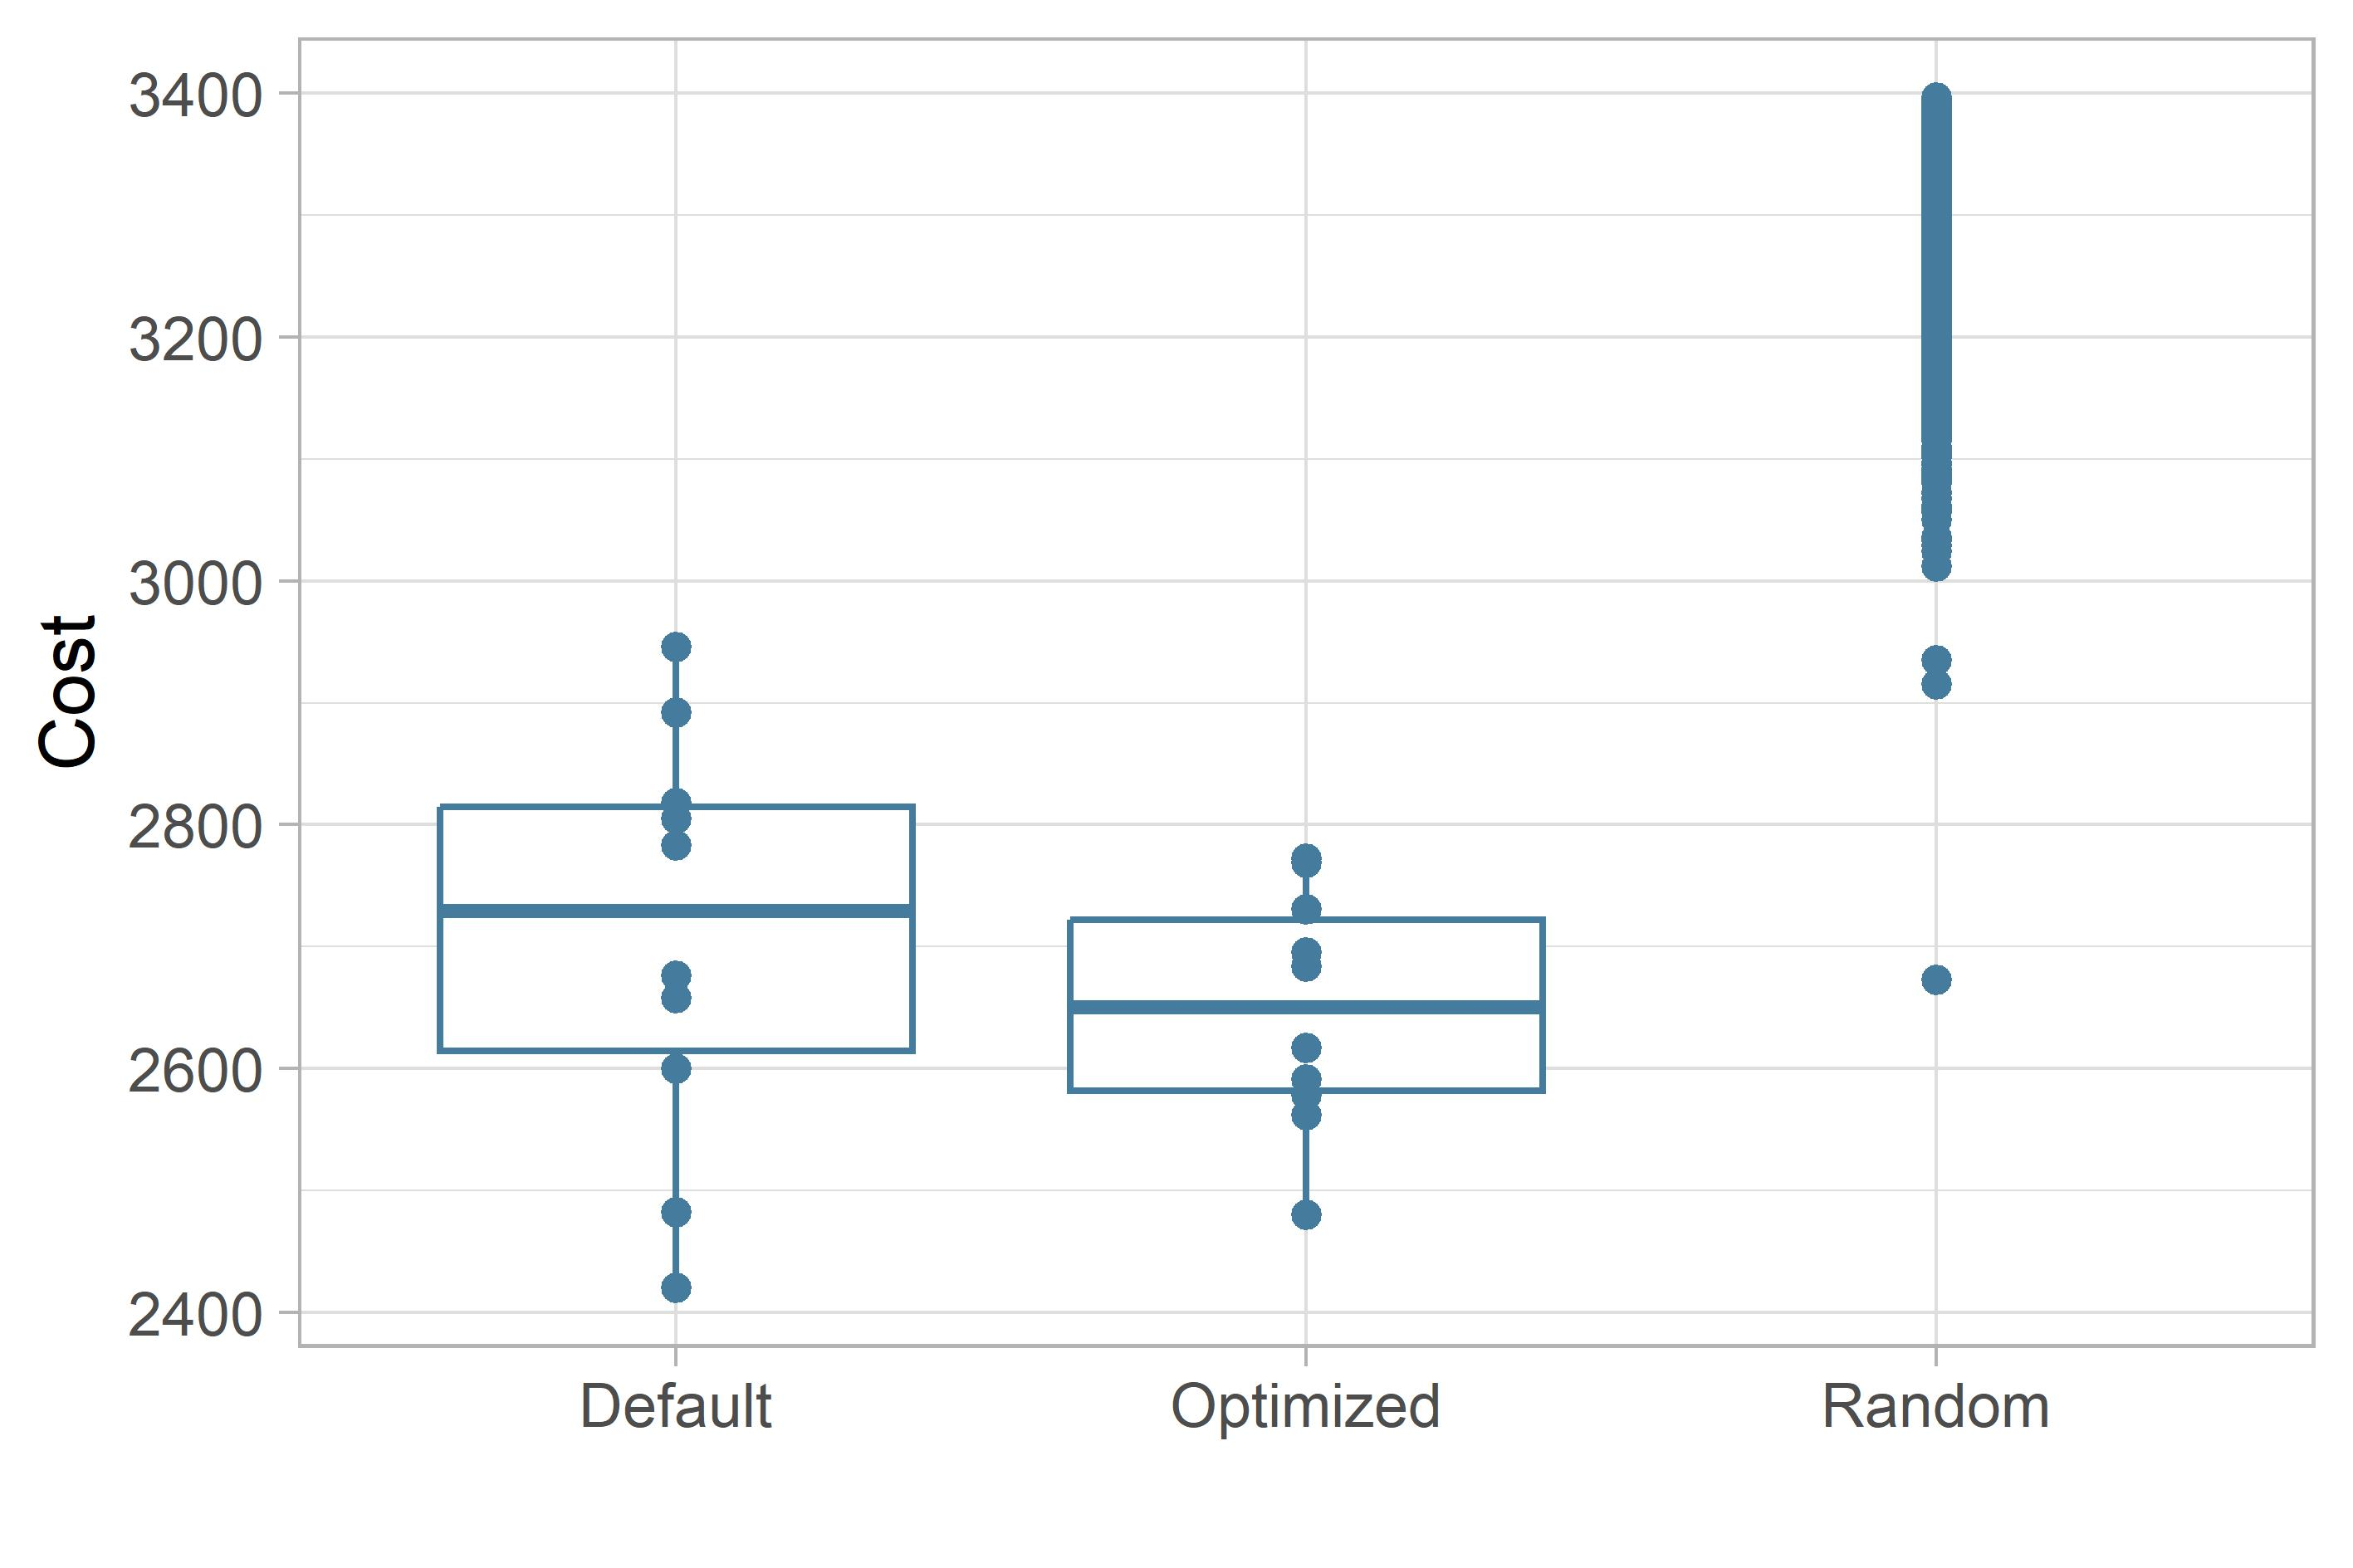
\includegraphics[width=1\linewidth]{simulations/evaluation/plots/sim_1_comparison}
	\caption{Genetic Algorithm with Elite}
\end{figure}


\section{Start Scenario 3}
Start Scenario 3 is described in more detail in \todo{ref}. 5 vehicles with 3 pedestrians are initialized, resulting in the simulation with the least NPCs.








\begin{figure}[ht] 
	\label{figure:sim_3_comparison}
	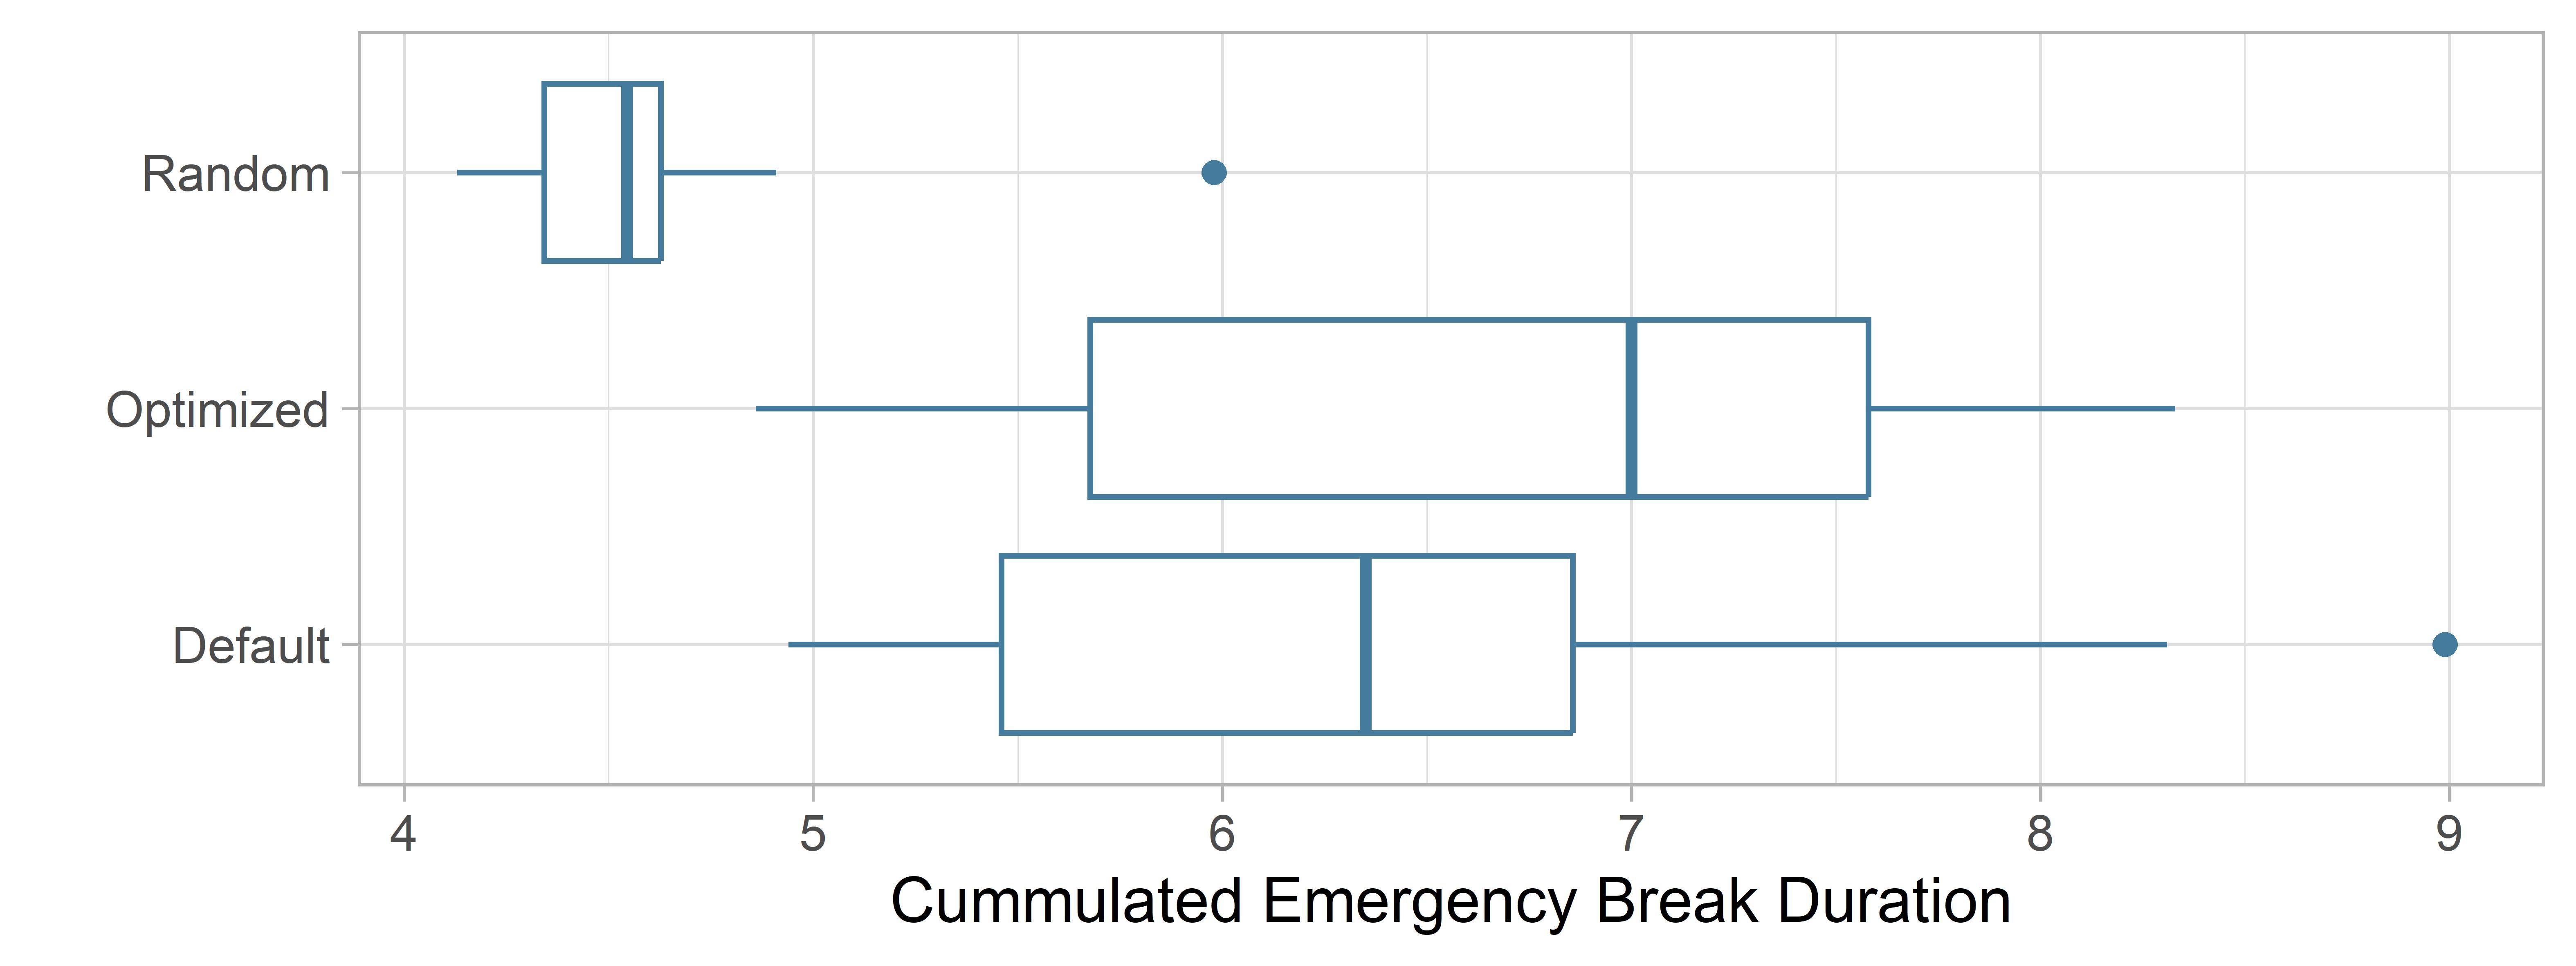
\includegraphics[width=1\linewidth]{simulations/evaluation/plots/sim_3_comparison}
	\caption{Start Scenario 3: Default GA vs Optimized GA vs Random Search}
\end{figure}

Looking at the graph, the Optimized Algorithm clearly outperformed the Default GA as well as Random Search.

The Two Sample t-test shows the same picture when comparing both GA algorithms. On average, greater fitness is achieved by using Optimized GA (M = 6.66, SE = ?) than from using Default GA (M = 6.49, SE = ?). This difference was however not significant \textit{t}(17.83) = -0.92, p > .05. No effect r = 0.07 \todo{How to call it exaclty?} complements these findings.

To further analyse both genetic algorithms, a look at their performance over the generations next to their diversity chart is of interest. Figure \ref{figure:sim_3_ga_comparison} plots the mean over the 10 repetitions, the outline show the min and max values.

\begin{figure}[ht] 
	\label{figure:sim_3_ga_comparison}
	\begin{minipage}[b]{0.5\linewidth}
		\centering
		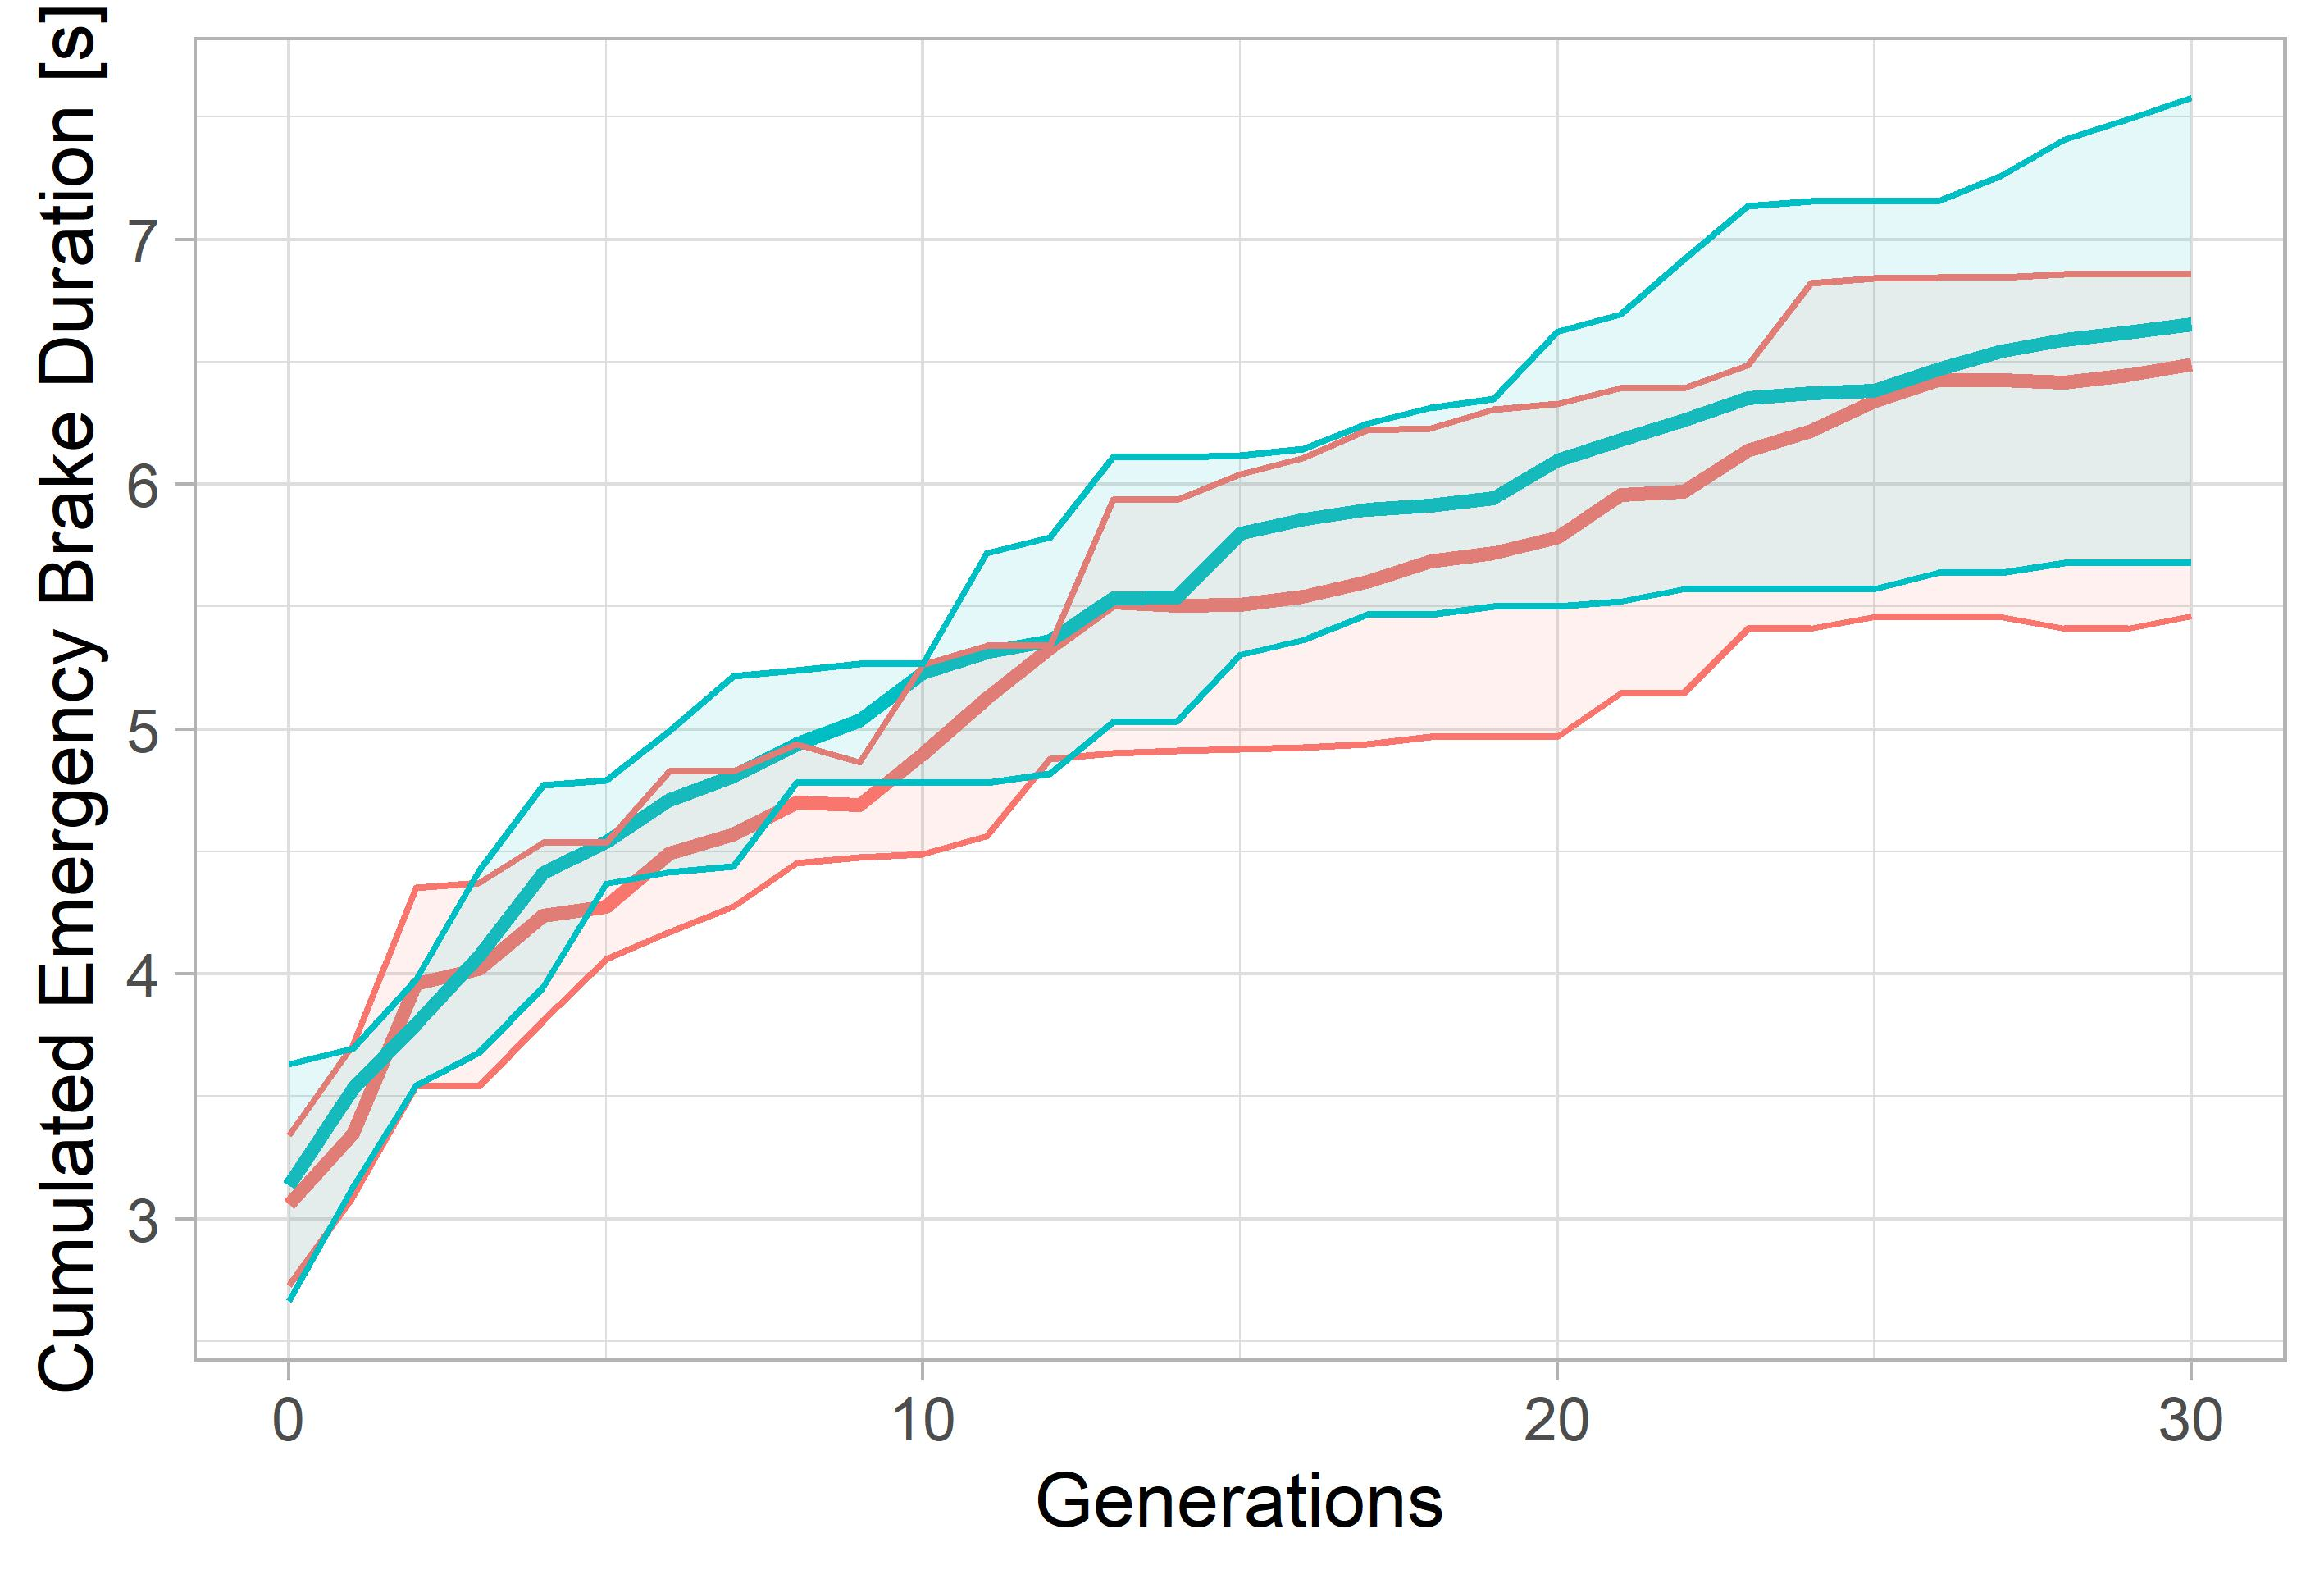
\includegraphics[width=1\linewidth]{simulations/evaluation/plots/sim_3_ga_generations} 
	\end{minipage}%%
	\begin{minipage}[b]{0.5\linewidth}
		\centering
		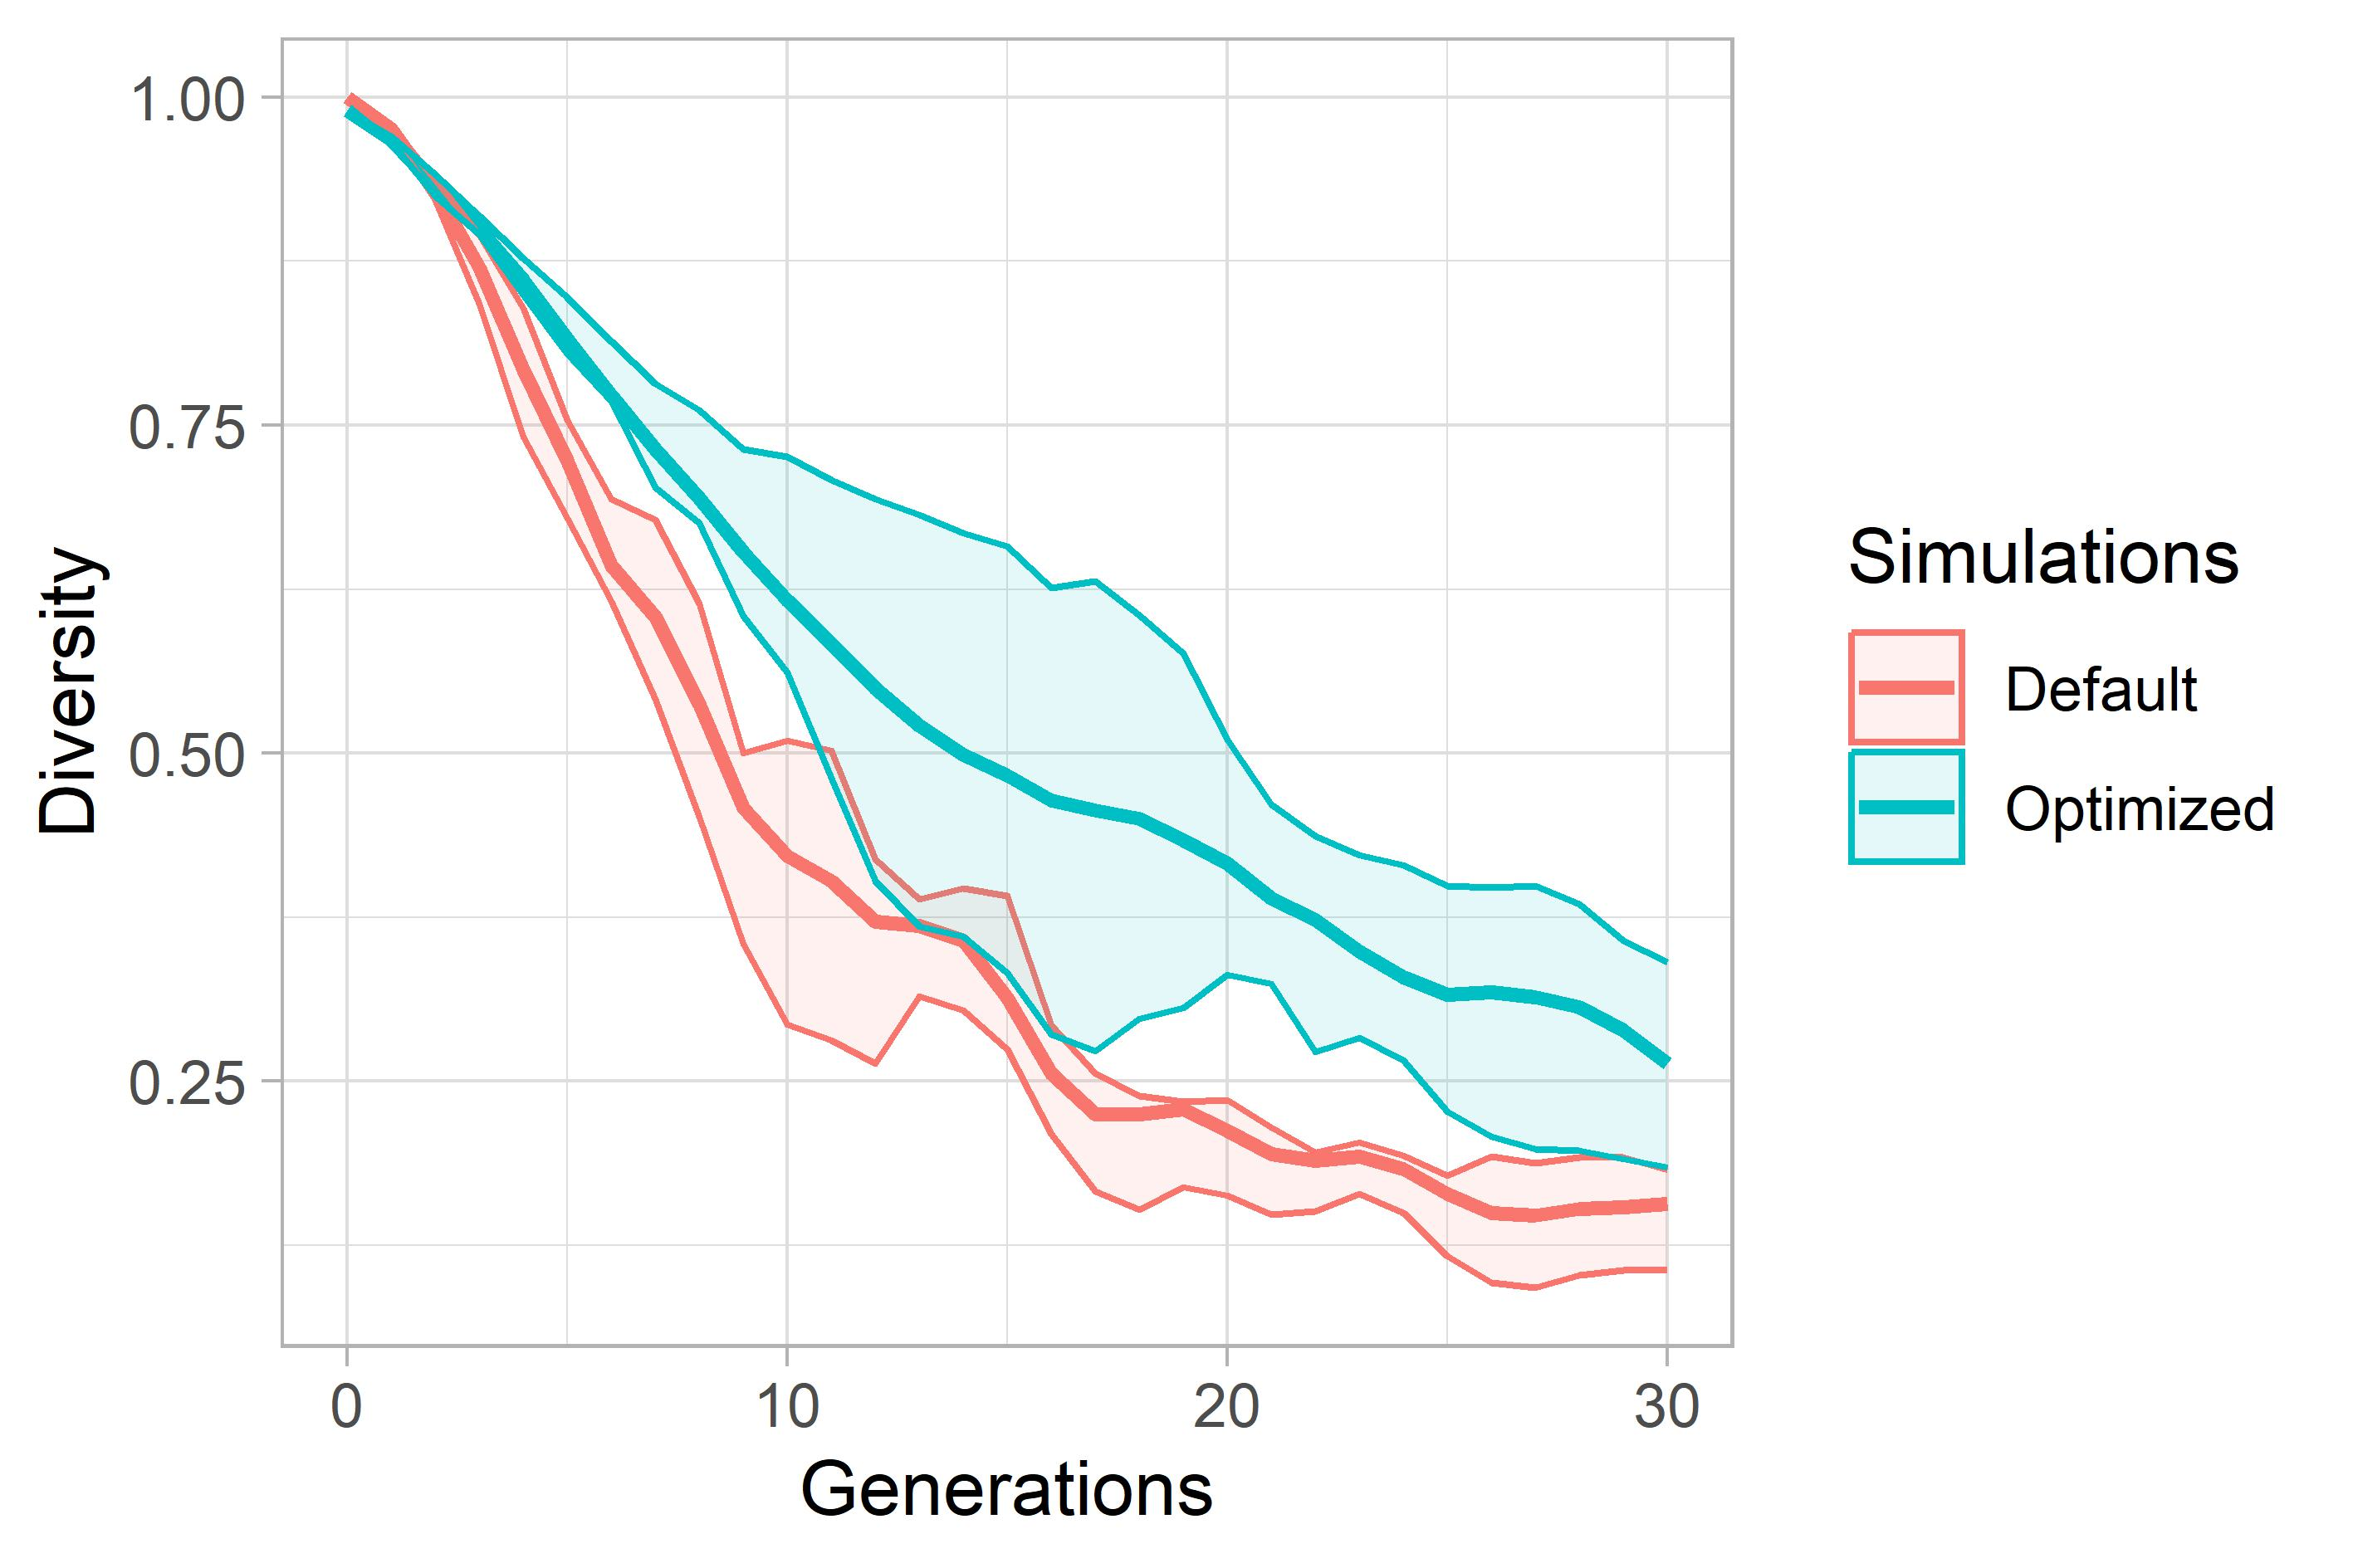
\includegraphics[width=1\linewidth]{simulations/evaluation/plots/sim_3_ga_diversity} 
	\end{minipage} 
	\caption{Start Scenario 3: Comparison of GAs}
\end{figure}


The rate of improved fitness of the Default GA drops is very similar to the Optimized one. Also the early decline in the diversity is not as pronounced as in the previous two comparisons. While the optimized GA shows to still hold the diversity in the population longer, this only improves its average fitness in a minimal manner.

Imagining a reason for this similar performance is difficult, on explanation might be the smaller search space due to the smaller number of NPCs. Now the high mutation and crossover rates might not have the huge advantage compared to previously.

Unsurprisingly due to the low number of NPCs, the cumulated emergency break time is on average lower compared to the other simulations.

\section{Start Scenario 4}
Start Scenario 4 is described in more detail in \todo{ref}. 18 vehicles with 10 pedestrians are initialized, resulting in the simulation with the most NPCs.

\begin{figure}[ht] 
	\label{figure:sim_4_comparison}
	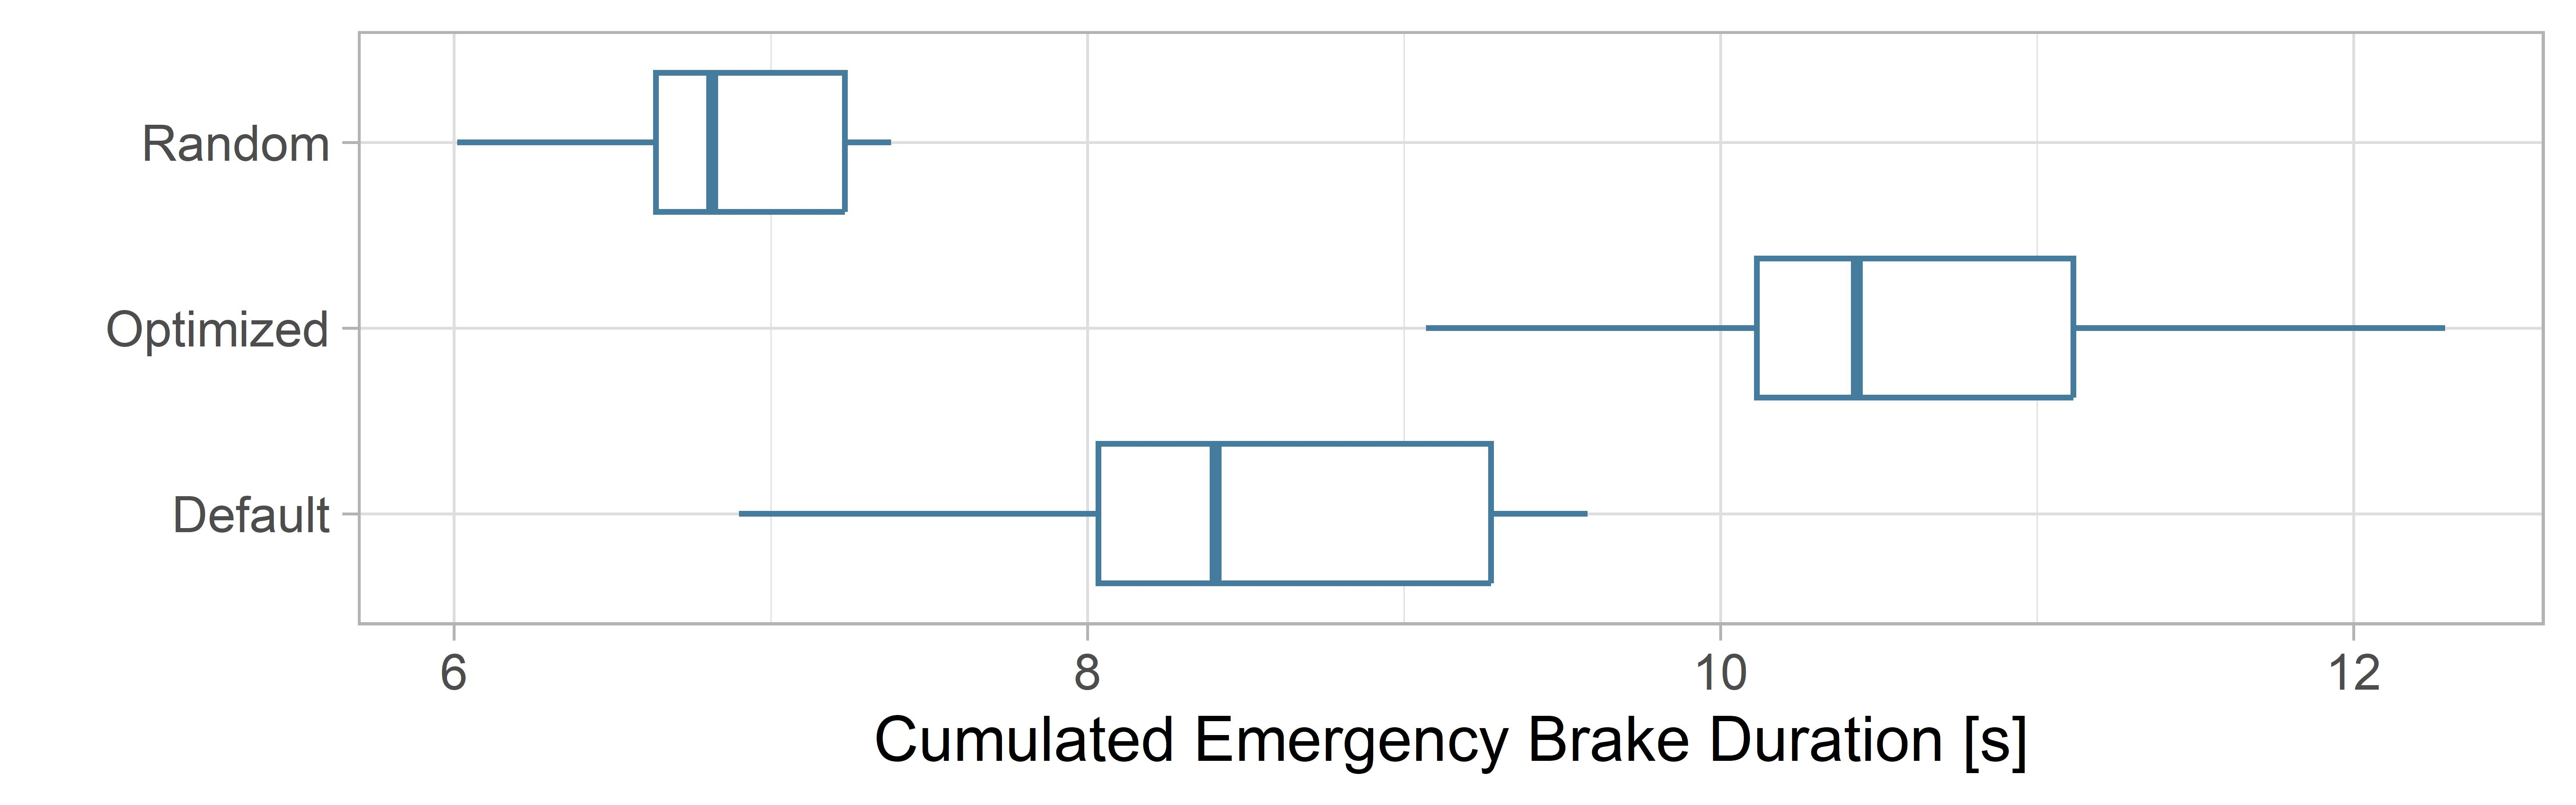
\includegraphics[width=1\linewidth]{simulations/evaluation/plots/sim_4_comparison}
	\caption{Start Scenario 4: Default GA vs Optimized GA vs Random Search}
\end{figure}

Looking at the graph, the Optimized Algorithm clearly outperformed the Default GA as well as Random Search.

The Two Sample t-test shows a clear result when comparing both GA algorithms. On average greater fitness is achieved by using Optimized GA (M = 10.60, SE = ?) than from using Default GA (M = 8.46, SE = ?). This difference was significant \textit{t}(17.98) = -5.30, p < .05. It did represented the largest effect r = 0.78.

COMP TO RAND
	Welch Two Sample t-test

data:  value by simulation
t = 11.706, df = 12.727, p-value = 3.504e-08
alternative hypothesis: true difference in means between group Optimized and group Random is not equal to 0
95 percent confidence interval:
3.052328 4.437672
sample estimates:
mean in group Optimized    mean in group Random 
10.600                   6.855 

[1] "Effect Size:"

[1] 0.957

To further analyse both genetic algorithms, a look at their performance over the generations next to their diversity chart is of interest. Figure \ref{figure:sim_4_ga_comparison} plots the mean over the 10 repetitions, the outline show the min and max values.

\begin{figure}[ht] 
	\label{figure:sim_4_ga_comparison}
	\begin{minipage}[b]{0.5\linewidth}
		\centering
		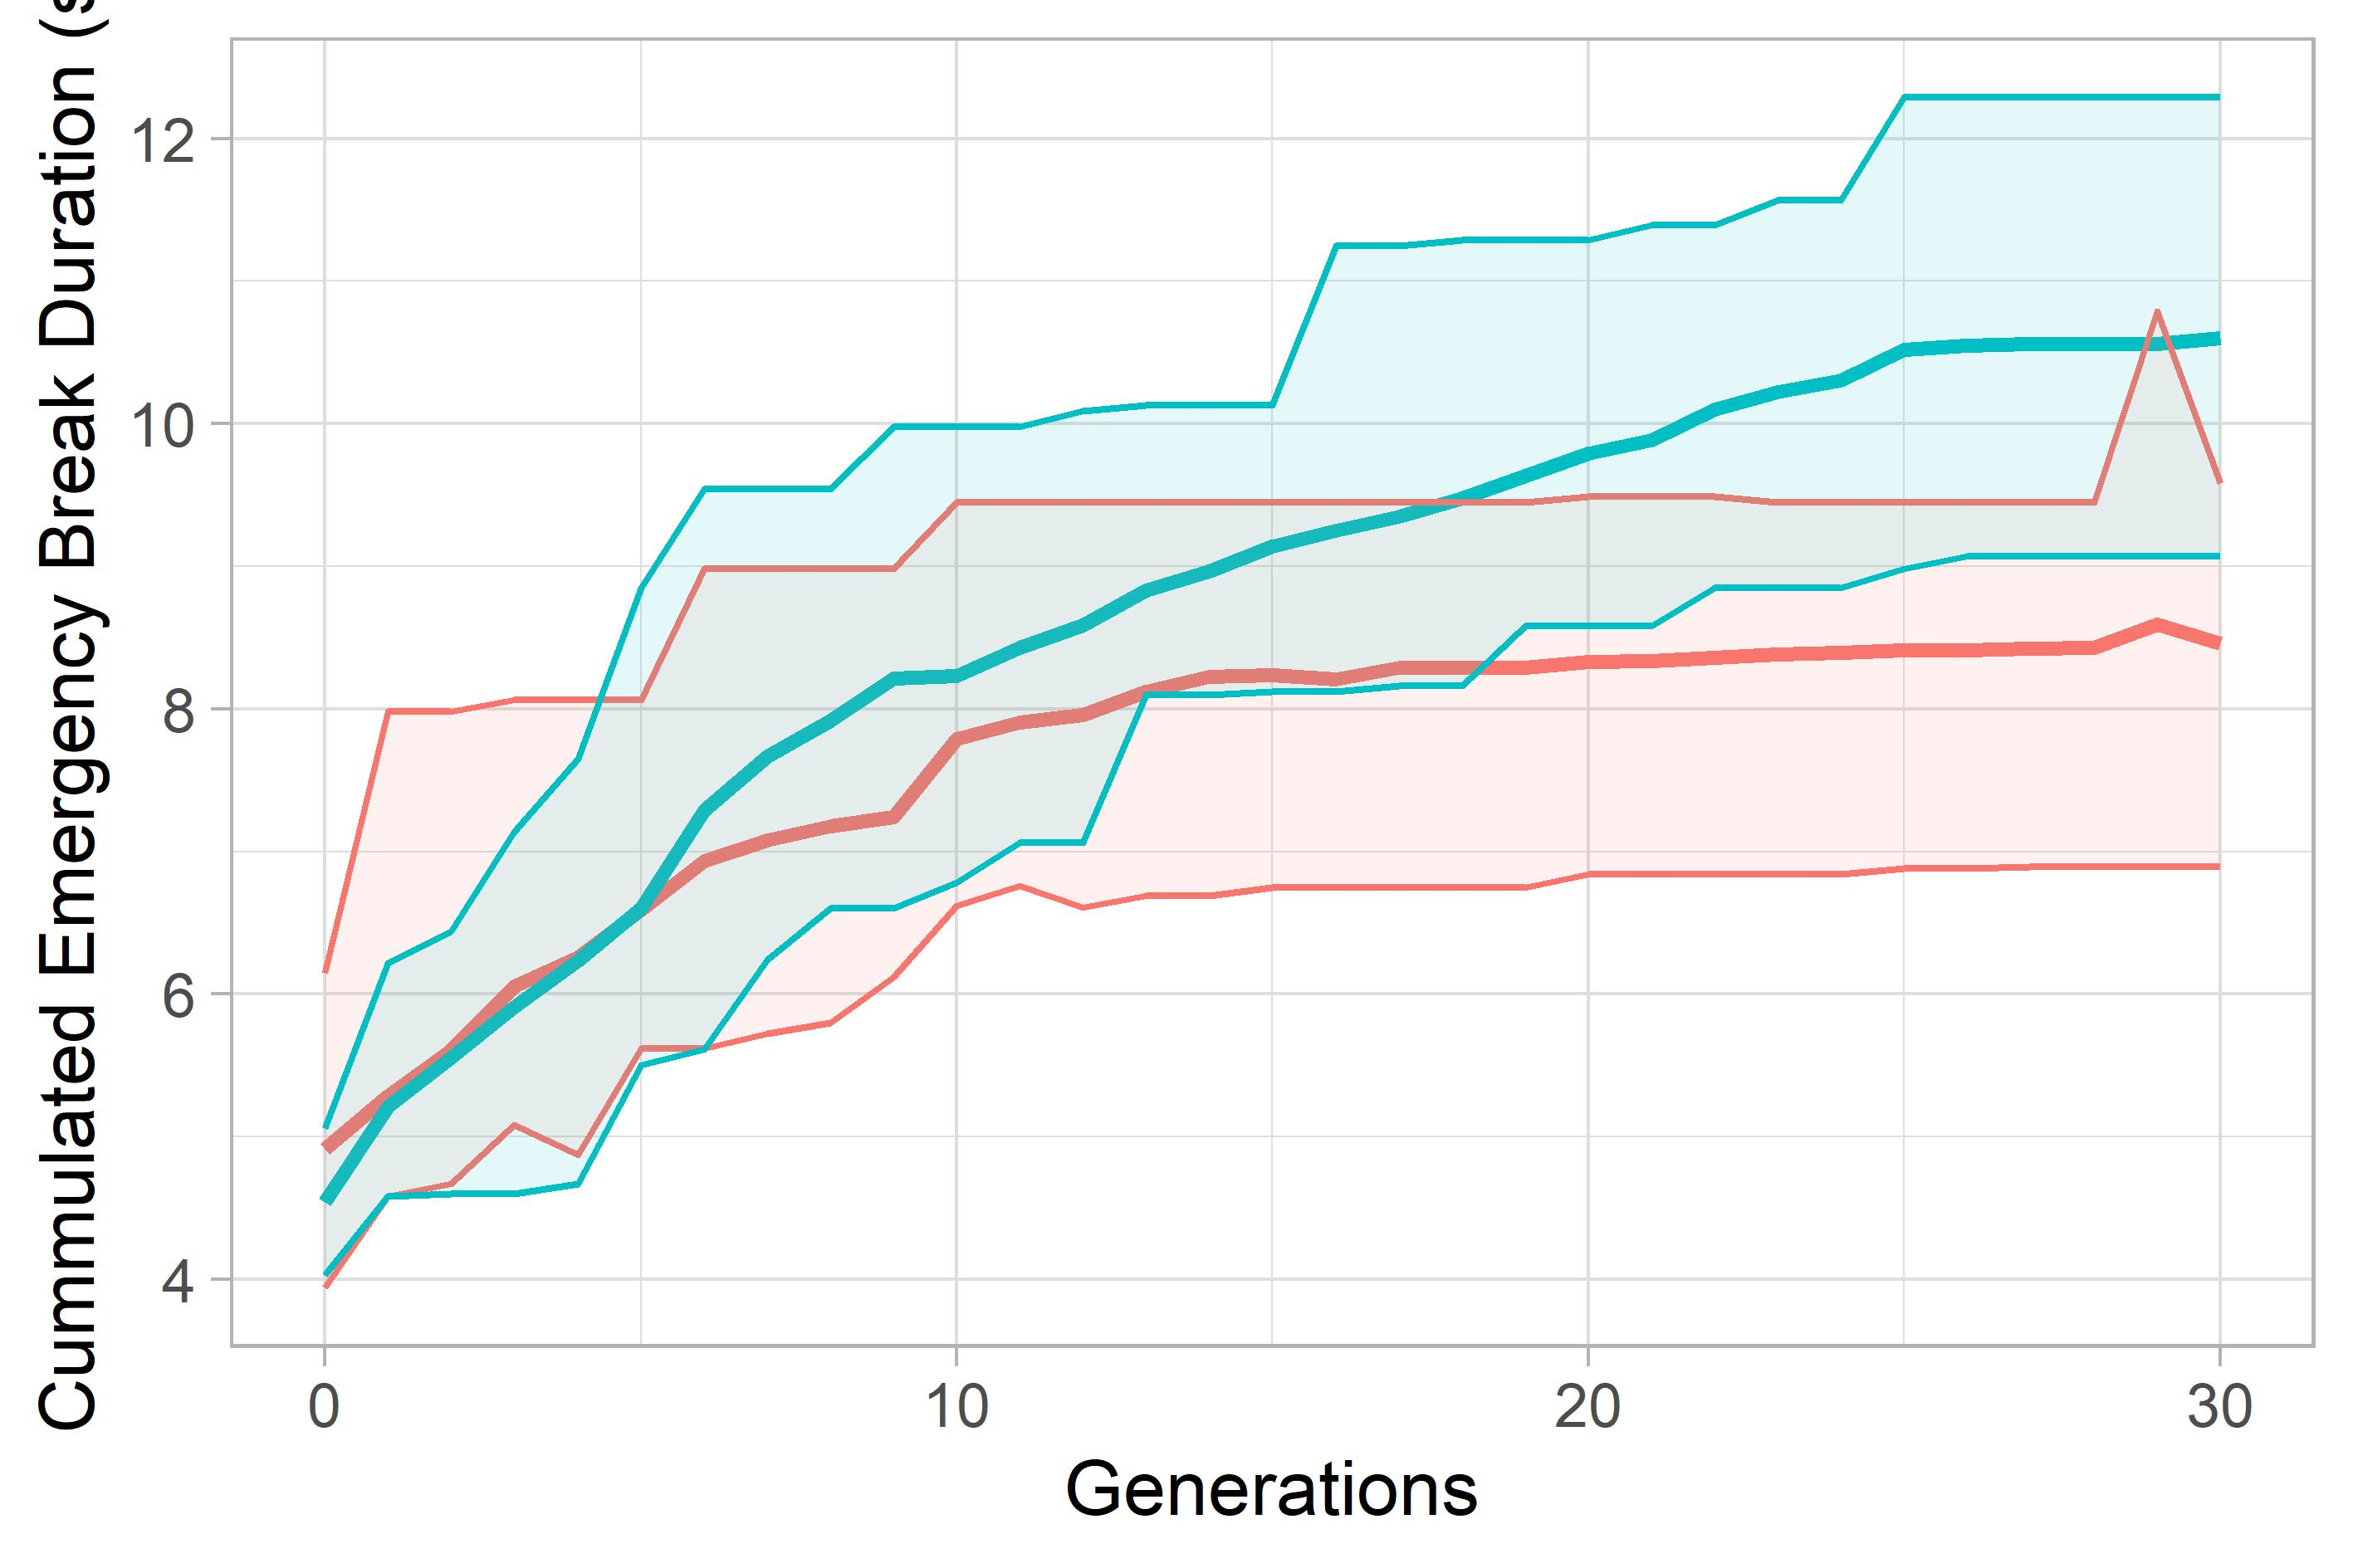
\includegraphics[width=1\linewidth]{simulations/evaluation/plots/sim_4_ga_generations} 
	\end{minipage}%%
	\begin{minipage}[b]{0.5\linewidth}
		\centering
		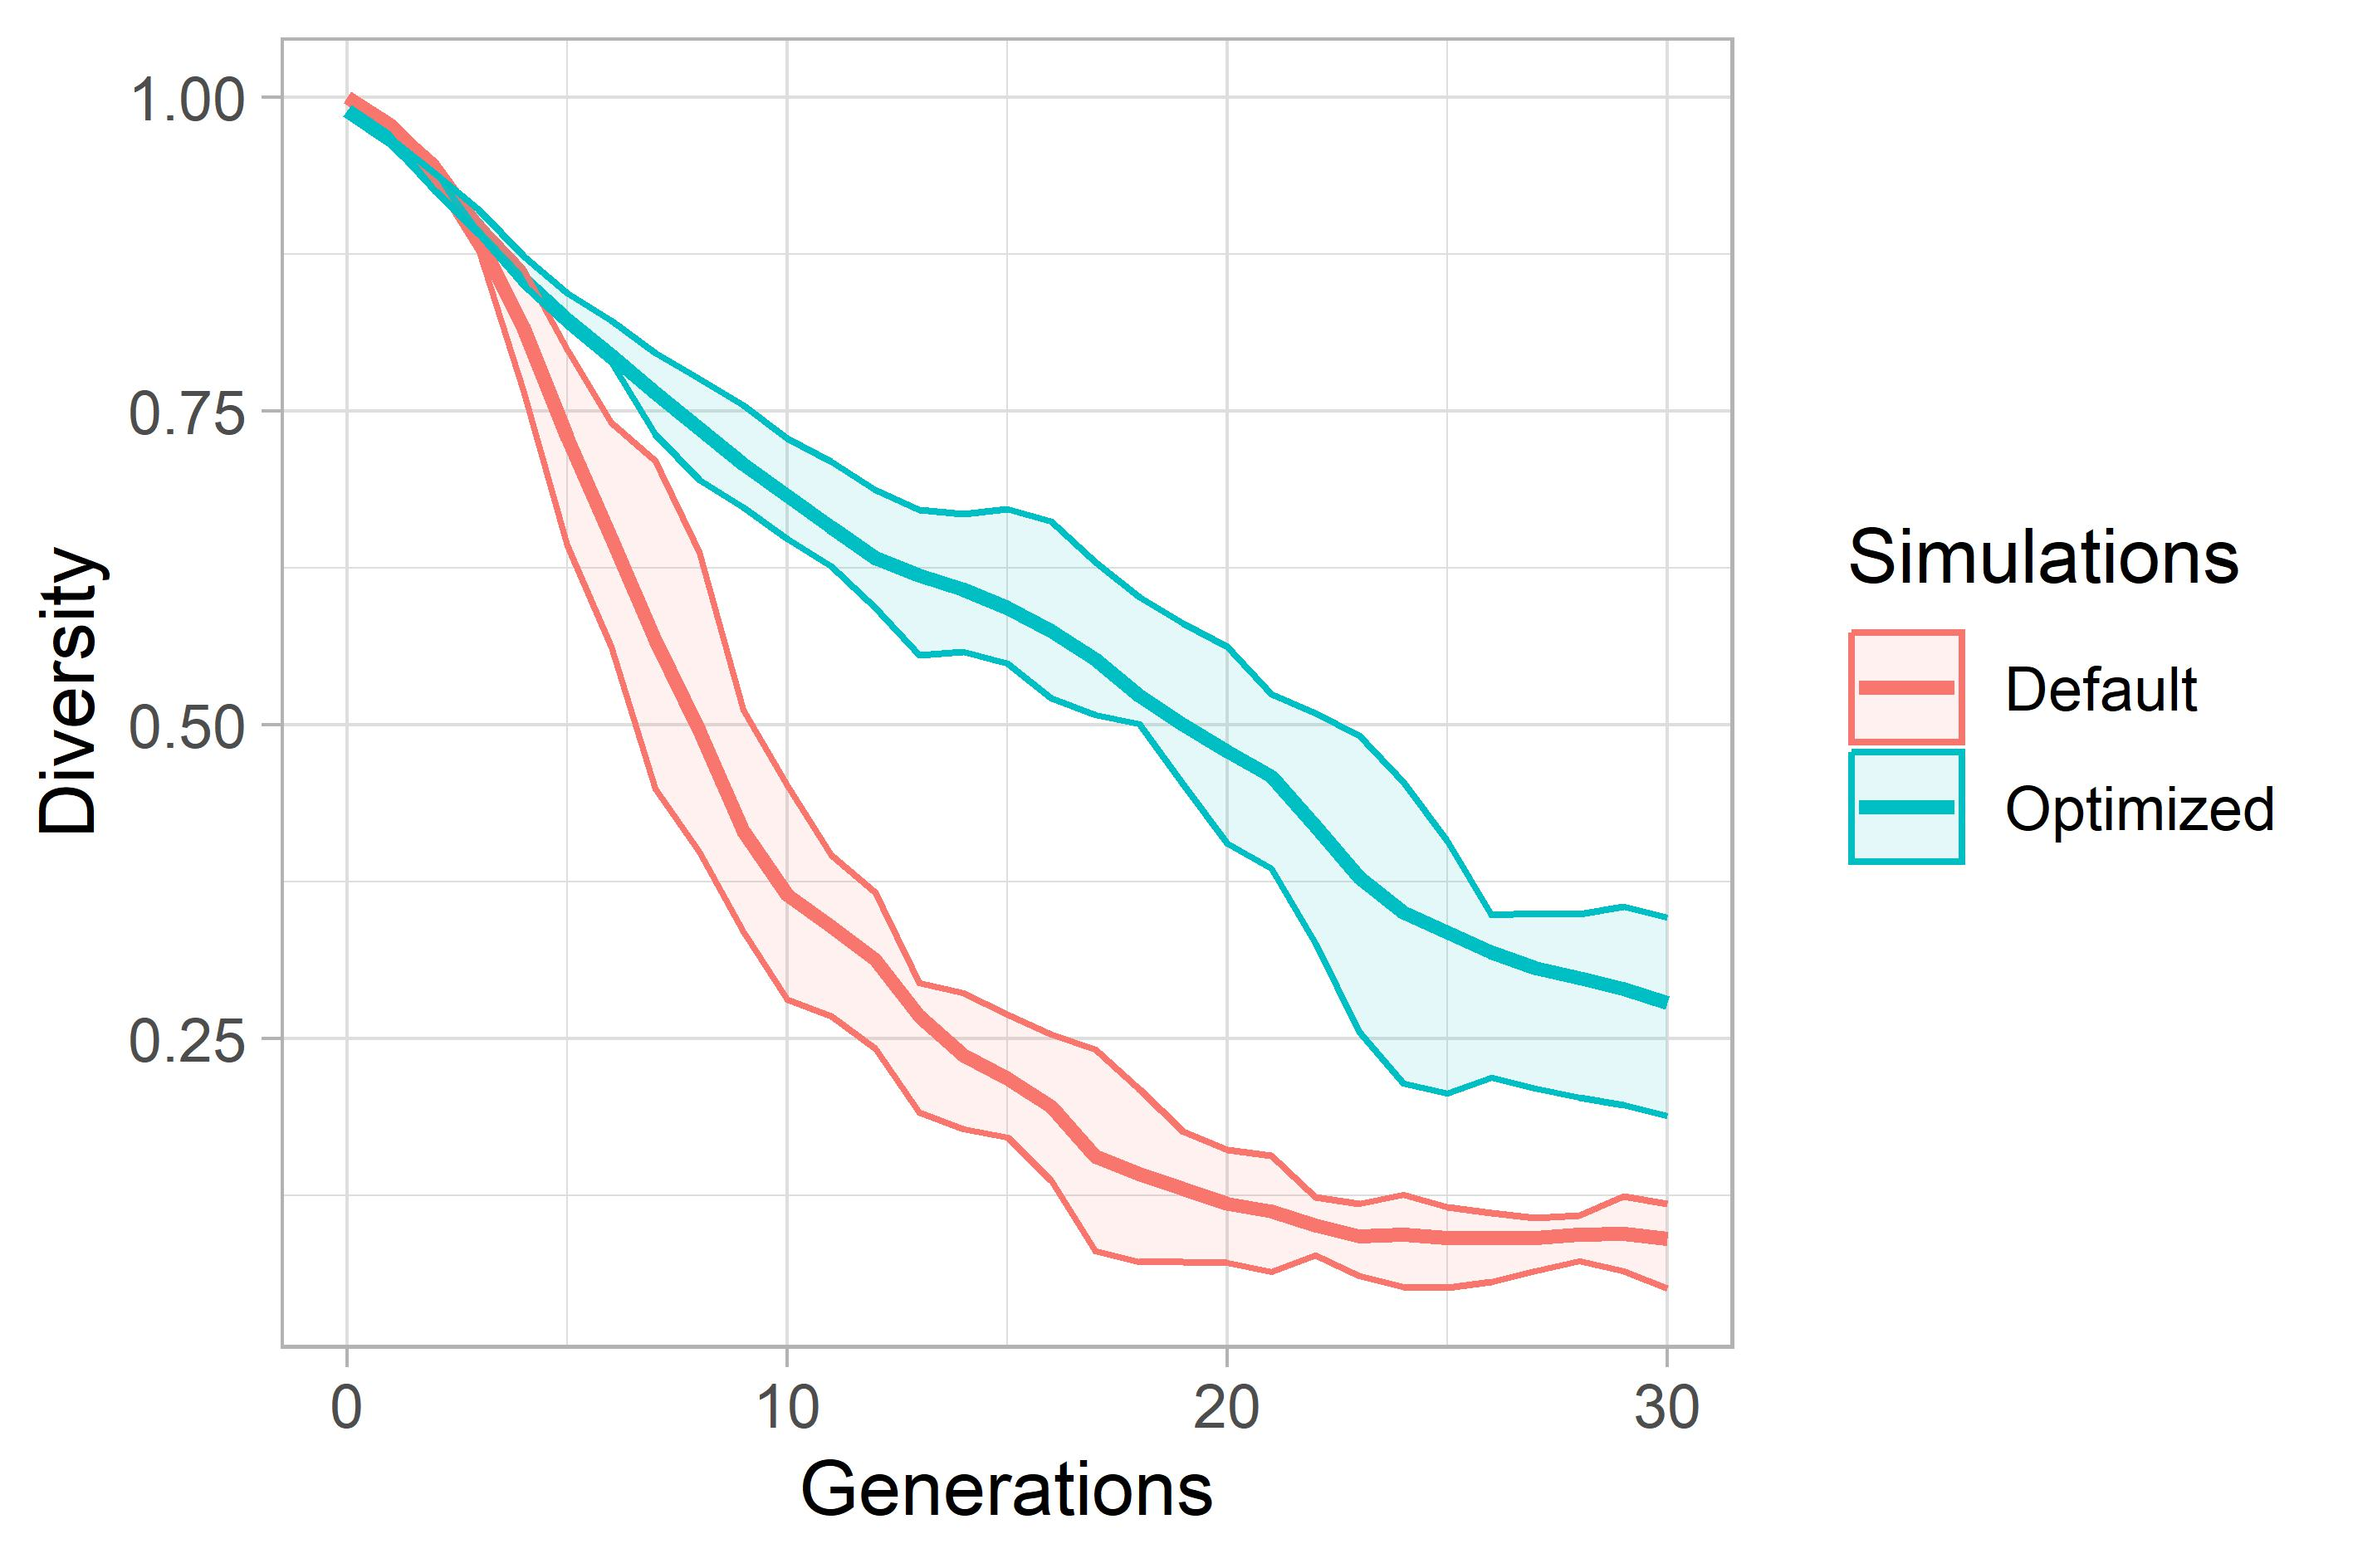
\includegraphics[width=1\linewidth]{simulations/evaluation/plots/sim_4_ga_diversity} 
	\end{minipage} 
	\caption{Start Scenario 4: Comparison of GAs}
\end{figure}


Already at generation 5, the rate of improved fitness of the Default GA drops compared to the Optimized one. A combined with an early sharp decline in the diversity, suggests a connection. The optimized GA shows to hold the diversity in the population longer, its rate of convergence is linear.